\documentclass[14pt,a4paper]{scrartcl}
\renewcommand{\sfdefault}{cmr}

\usepackage[utf8]{inputenc}
\usepackage[english,russian]{babel}

\usepackage{hyperref}
\usepackage{indentfirst}
\usepackage{misccorr}
\usepackage{graphicx}
\usepackage{amsmath}
\usepackage{amssymb}
\usepackage{amsfonts}
\usepackage{alltt}
\usepackage{enumitem}
\usepackage{xcolor}


\begin{document}
\section{Вопрос 1}
\subsection{\textbf{Основы квантово-механической теории строения атома в контексте образования химической связи.}}

 В соответствии с волновой механикой, какая-либо микросистема
описывается функцией состояния, или волновой функцией, которая
является функцией координат всех частиц, образующих эту систему
и от времени, если эта система находится не в стационарном
состоянии. Вероятность нахождения частицы в бесконечно малом
объёме пропорциональна квадрату $\psi^2$ ее волновой функции или
произведению $\psi\cdot\psi$, где $\psi*$ - комплексно-сопряженная $\psi$, если
волновая функция - комплексная величина. Как и другие волны,
волновая функция имеет области положительных и отрицательных
амплитуд, но знак не имеет физического смысла, если в одной
области пространства есть только одна волновая функция. Если же
их две, знак волновой функции имеет чрезвычайно важное
значение.

В результате их интерференции аплитуда
результирующей волновой функции может либо повыситься, если
исходные волновые функции имели одинаковые знаки в данной
области, либо понизиться, если волновые функции имеют
противоположные значения.

Термин «химическая связь» не имеет строгого определения. Для
ковалентных соединений с позиций квантовой механики это есть
результат взаимодействия нескольких волновых функций. Согласно
методу валентных связей, волновая функция электронной пары
формируется путем наложения волновых функций для отдельных
фрагментов молекулы, то есть является суперпозицией волновых
функций каждой конфигурации. Образование связи можно
представить как высокую вероятность нахождения двух электронов
между двумя ядрами. Например, связь в молекуле водорода
описывается следующим образом. Были выбраны орбитали
каждого атома с одним электроном $(\psi(A)$ и $\psi(B))$, и
соответствующие волновые функции объединяют в волновую
функцию одновременно двух электронов.

$$\psi = \psi_A(1)\cdot\psi_B(2) + \psi_B(1)\cdot\psi_A(2)$$

Эту операцию называют спариванием электронов, что является процессом с проигрышем энергии.

С позиции метода молекулярных орбиталей, движущей силой образования ковалентной связи является делокализации электронов. Одноэлектронные функции - молкулярные орбитали, каждую из которых можно рассмотреть как линейную комбинацию атомных орбиталей -- сумму атомных орбиталей с различными коэффициентами. Пример для $H_2$:

$$\psi = C_A\varphi_A + C_B\varphi_B$$

$$1) C_A =  CB= 1;  \psi_+ = \varphi_A + \varphi_B$$

Связывающая орбиталь. Связывающий характер объясняется интерференцией двух атомных орбиталей с одинаковыми по знаку амплитудами, что является причиной повышения амплитуды волновой функции между ядрами. Электрон, занимающий эту орбиталь, с повышенной вероятностью находится в межъядерном пространстве и может сильнее взаимодействовать с обоими ядрами.

$$C_A =1; C_B = -1; \psi_- = \varphi_A-\varphi_B$$

Разрыхляющая орбиталь. Большая энергия электрона на этой орбитали
возникает вследствие интерференции двух атомных орбиталей с разными по
знаку амплитудами, при этом амплитуды волновых функций вычитаются и
между двумя ядрами образуется узловая плоскость.

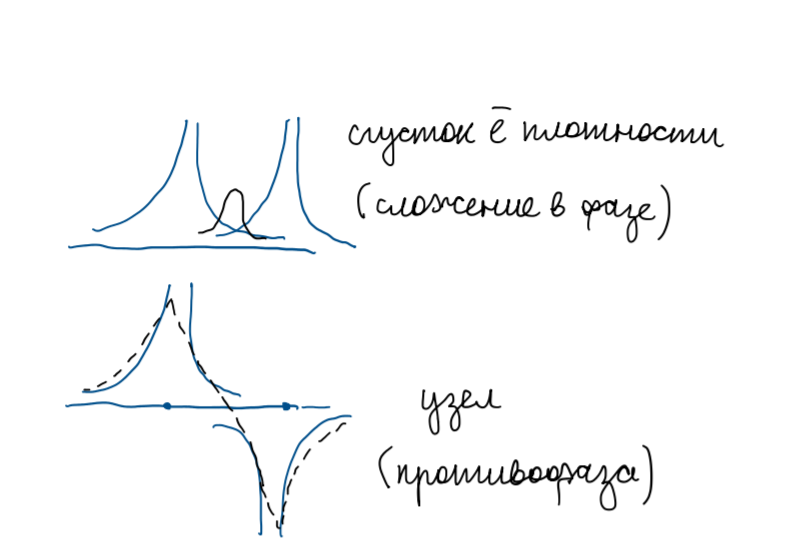
\includegraphics[scale=0.7]{1v.png}

\subsection{\textbf{Ионная связь. Строение ионных соединений в твердой фазе и в растворе.}}

В основе ионных соединений лежит кулоновское взаимодействие. У
ионных кристаллов в узлах решётки находятся положительные и
отрицательные ионы, в отличие от атомов или молекул в узлах
ковалентных кристаллов. Ионы в узлах ионного кристалла
расположены таким образом, что силы притяжения между
разнозаряженными ионами максимальны, а силы отталкивания
между одинаково заряженными ионами минимальны. 

Согласно модели жёстких сфер, ионы рассматриваются как практически
несжимаемые жёсткие сферы, почти не смещающиеся со своих
позиций. Невозможно обнаружить сходство свойств иона и атома,
образовавшего этот ион. Свойства катиона не зависят от свойств
аниона и наоборот. В ионных соединениях невозможно выбрать
направление связи, нет валентных углов. Основные требования при
образовании ионных соединений заключаются в том, что атомы
металла должны иметь относительно низкий потенциал
ионизации, а атомы неметаллов или радикалы - сравнительно
высокое сродство к электрону. 

В состав ионного соединения должны входить элементы с сильно различающимися
значениями электроотрицательности. Общая электронная пара
локализуется у атома с большей электроотрицательностью. В
отличие от ковалентной связи, разделение зарядов практически
полное. 

Тем не менее, ионных на 100 процентов соединений не существует,
поскольку за «идеал» ионного взаимодействия берётся связь
протона и электрона, там разделение зарядов 100-е. 

Степень разделения зарядов можно определять по величине
дипольного момента молекулы, который измеряется в Дебаях (Д).
Помимо кулоновского притяжения двух находящихся рядом
противоположно заряженных ионов, будет осуществляться и
взаимодействие, обусловленное взаимной поляризацией. Чем
меньше по размеру и более высоко заряжен катион, тем больше он
будет стремиться нарушить распределение заряда в соседнем
анионе. Поляризуемость аниона растет с ростом его размера и
заряда (по модулю). В основном смотрят на деформацию именно
анионов катионами, а не наоборот, поскольку анионы по размеру
больше катионов. Если при ионной связи поляризация анионов
настолько велика, что дает заметное увеличение электронной
плотности между ядрами, то уже можно рассматривать это как
случай ковалентной связи.

\subsubsection{\textbf{Строение и свойства ионных соединений в твердой фазе}}

Представляют собой бесконечную периодическую решётку. В
идеале, кристалл состоит из бесконечного количества
элементарных ячеек. В твёрдой фазе очень много ионных
взаимодействий. Электрическая проводимость чаще всего низкая,
потому что ионы в узлах решётки закреплены и не могут свободно
перемещаться. Ионные соединения имеют высокие температуры
плавления, потому что ионные связи обычно сильны и
ненаправленны (распространяются во всех направлениях). Ионные
соединения обычно твёрдые, но хрупкие. Твёрдость объясняется
невозможностью образования кратных связей вследствие
разделения ионов в пространстве и отсутствия теплового движения
ионов. Хрупкость объясняется природой ионной связи: даже при
относительно небольшом сдвиге ионов возникают контакты анионанион и катион-катион и вместо сил притяжения появляются силы
отталкивания, вследствие чего кристалл раскалывается.

\subsubsection{\textbf{Пример проявления поляризации}}

$$CaF_2 - CaCl_2 - CaBr_2 - CaI_2$$

В этом ряду слева направо уменьшается температура
плавления соединения, потому что увеличиваются
радиусы анионов, что увеличивает их
поляризуемость. Это снижает энергию
кристаллической решётки, так что для расплавления
вещества требуется меньше энергии.

\subsubsection{\textbf{Строение и свойства ионных соединений в растворе}}

Ионные соединения в растворе взаимодействуют с полярными
молекулами растворителя. За счёт большой энергии сольватации
происходит выигрыш в энергии. В растворе можно обнаружить
следующие ассоциаты:


1) Сольватированные ионы( реально встречаются только при низких концентрациях)

$$M^+(solv) - - - - -X^-(solv)$$

2) Сольватно-разделенные ионные пары(сольватированные ионы разделены молекулой растворителя)

$$M^+(solv) || X^-(solv); ||=(solv)$$

3) Контактные ионные пары

$$(solv)M^+X^-(solv)$$

В растворе ионные соединения имеют высокую проводимость,
поскольку в этих веществах имеются ионы, которые могут
свободно двигаться под действием электрического поля. Ионные
соединения заметно растворимы в полярных растворителях с
высокой диэлектрической проницаемостью. Энергия
взаимодействия двух заряженных частиц в некоторой среде обратно
ей пропорциональна:


$$E = \frac{q^+q^-}{4\pi\epsilon r}$$

\subsection{\textbf{Различные методы описания ковалентной связи.}}

В ковалентных соединениях молекулы обособлены, то есть любые
внутримолекулярные взаимодействия много сильнее, чем
межмолекулярные. Также могут быть определены межатомные
радиусы. Отличия от ионной связи:
 
1) Направленность  (способность атома выбирать себе направление
для смещения электронной плотности)

2) Насыщаемость (способность образовывать определенное
количество связей)

Из первого отличия следует, что для ковалентных связей можно
изучить некоторые геометрические характеристики: длина связи,
валентные и торсионные углы.

Для образования химической связи орбитали должны быть
способными перекрыться по симметрии, энергии их должны быть
довольно близки, должно наблюдаться сближение в пространстве.

В методе валентных связей движущей силой образования химической
связи является обобществление электронов и образование
электронных пар. Тем не менее, важно помнить, что спаривние
электронов - это очень невыгодный процесс. Метод валентных связей
не может объяснить некоторые молекулы. Например, в $PCl_5$ у
фосфора реально 10 электронов, а не 8 (МВС можно рассматривать как
выражение идей Льюиса в терминах волновой механики, а по
Льюису каждый атом делит электроны с соседним атомом для
достижения полной валентной оболочки с восемью электронами); в
молекуле кислорода по МВС все электроны спарены, хотя эта
молекула - бирадикал.

 Согласно методу валентных связей, волновая
функция электронной пары формируется путем наложения волновых
функций для отдельных фрагментов молекулы, то есть является
суперпозицией волновых функций каждой конфигурации.
Образование связи можно представить как высокую вероятность
нахождения двух электронов между двумя ядрами. Например, связь в
молекуле водорода описывается следующим образом. Были выбраны
орбитали каждого атома с одним электроном ($\psi(A)$ и $\psi(B)$), и
соответствующие волновые функции объединяют в волновую
функцию одновременно двух электронов.

$$\psi = \psi_A(1)\cdot\psi_B(2) + \psi_B(1)\cdot\psi_A(2)$$
 
 В соответствии с принципом Паули эта волновая функция может
описывать только электроны со спаренными (разными) спинами,
поэтому в МВС только спаренные электроны могут участвовать в
спаривании. Когда происходит спаривание спинов, возникают силы
притяжения, и образуется электронная пара связи.

Эту волновую функцию можно «улучшать» и дальше, учитывая
экранирование ядер и ионное распределение электронов к какомулибо одному атому, но она никогда не достигнет такого улучшения,
при котором расчетная энергия окажется равной истинному
значению энергии системы.

Метод молекулярных орбиталей исходит из того, что движущей
силой образования химической связи является делокализация
электронов (это выигрышный по энергии процесс). Он основан на
допущении, что связывающие электроны находятся в молекуле на
молекулярных орбиталях, как в атоме - на атомных. 

Принимается возможность образования
молекулярных орбиталей при линейной комбинации атомных
орбиталей (ЛКАО-МО). Если в поле двух атомных ядер А и Б
находится один электрон, то он может находиться то у одного ядра,
то у другого. Суперпозиция этих состояний может быть выражена с
помощью ЛКАО.

$$\psi = \psi_A + \psi_B$$
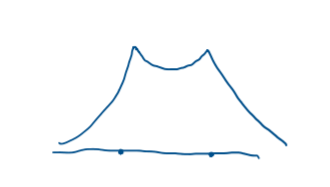
\includegraphics{3v1.png}

\textbf{Связывающая орбиталь.} Связывающий характер объясняется интерференцией двух атомных
орбиталей с одинаковыми по знаку амплитудами, что является причиной повышения
амплитуды волновой функции между ядрами. Электрон, занимающий эту орбиталь, с
повышенной вероятностью находится в межъядерном пространстве и может сильнее
взаимодействовать с обоими ядрами. Когда эта орбиталь занята электронами, энергия
молекулы становится ниже, чем энергия изолированных атомов.

$$\psi^* = \psi_A - \psi_B$$
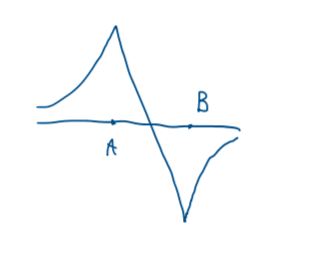
\includegraphics{3v2.png}

\textbf{Разрыхляющая орбиталь.} Большая энергия электрона на этой орбитали возникает
вследствие интерференции двух атомных орбиталей с разными по знаку амплитудами, при
этом амплитуды волновых функций вычитаются и между двумя ядрами образуется узловая
плоскость. Когда эта орбиталь занята электронами, энергия молекулы становится выше,
чем энергия отдельных атомов. Преобладает отталкивание между электронами $\Rightarrow$ 
ослабление связывания атомов. Разрыхляющая орбиталь всегда разрыхляет больше,чем
связывающая - связывает.

Важно, что по ММО для n атомных орбиталей получается n
молекулярных.

Для двухэлектронных систем волновая функция будет равна
произведению одноэлектронных волновых функций. Например,
для молекулы водорода.

$$\psi = \psi_1\cdot\psi_2 = (\psi_A(1)+\psi_B(1))(\psi_A(2)+\psi_B(2))$$

Вероятностное распределение электронной плотности пропорционально квадрату волновой функции:

$$\psi^2 = \psi_A^2 + 2\psi_A\psi_B + \psi_B^2$$
$$\psi^{*2} = \psi_A^2 - 2\psi_A\psi_B + \psi_B^2$$

Интеграл перекрывания:

$$S = \int\psi_a\psi_BdV$$

$$E\pm = \frac{E_F\pm\beta}{q\pm S}$$

$E_A = E_B$ - исходный уровень\\
$\beta$ - резонансный интеграл\\
$S$ - интеграл перекрывания

В области связывания интеграл перекрывания больше нуля, в
области разрыхления меньше нуля. Он также может быть равен
нулю для несвязывающих орбиталей. Чтобы образовалась связь,
должно доминировать положительное перекрывание.

На основании диаграмм молекулярных орбиталей можно
определить магнитные свойства молекулы, общий спин,
кислотность или основность по Льюису, увидеть способные к
донированию или акцептированию орбитали.

\subsection{\textbf{Соединения галогенов в степени окисления (-1), межгалогенные соединения, способы получения, химическое поведение, электронное и геометрическое строение молекул.}}

\subsubsection{Галогенводороды}

\textbf{Получение}

1) Прямой синтез из элементов

$$H_2 + X_2 = 2HX$$
($F_2, Cl_2$ -со взрывом, $Br_2, I_2$ - спокойнее, т.к. равновесие смещено влево)

2) Вытеснение HX из солей

$$CaF_{2(tv)} + H_2SO_{4(konc)} \rightarrow CaSO_4\downarrow + 2HF\uparrow$$
$$NaCl + H_2SO_{4(konc)} \rightarrow NaHSO_4 + HCl\uparrow$$
$$KX + H_3PO_{4(konc)} \rightarrow KH_2PO_4 + HX\uparrow$$

3) Гидролиз галогенидов неметаллов

$$SiCl_4 + 3H_2O \rightarrow H_2SiO_3 + 4HCl \uparrow$$
$$PX3 + 3H_2O  \rightarrow H_3PO_4 + 3HX\uparrow$$
$$2P_{kr} + 3X_2 + 6H_2O \rightarrow 2H_3PO_4 + 6HX$$

4) Галогенирование углеводородов

Побочные продукты при хлорировании и бромировании алканов и циклоалканов

5) Концентрированные кислоты

$$3Br_2 + S + 4H_2O \rightarrow H_2SO_4 + 6HBr$$
$$H_2S + I_2 \rightarrow 2HI + S\downarrow$$

\textbf{Химические свойства}

1) Кислоты в водных растворах

$$HX + HOH \rightleftharpoons X^- + H_3O^+$$
HF - слабая, HCl, HBr, HI - сильные, увеличение силы кислот

2) Восстановители (кроме HF)

$$MnO_{2(tv)} + 4HCl_{konc} \rightarrow MnCl_2 + 2H_2O + Cl_2$$

$$2HI + 2FeCl_3 \rightarrow 2FeCl_2 + I_2 + 2HCl$$

$$4HI + 2CuSO_4 \rightarrow2CuI\downarrow + I_2 + 2H_2SO_4$$

3) Азеотропные смеси с водой
 
4) Особые свойства HF

а) Водородные  связи

б) Образование гидрофторидов

$$HF + F^- \rightarrow HF_2^-$$
$[F-H-F]^-$ - линейный

в) с $SiO_2$

$$4HF{gas} + SiO_2 \rightarrow SiF_4\uparrow + 2H_2O$$

\textbf{Электронное и геометрическое строение молекул}

Линейные полярные молекулы

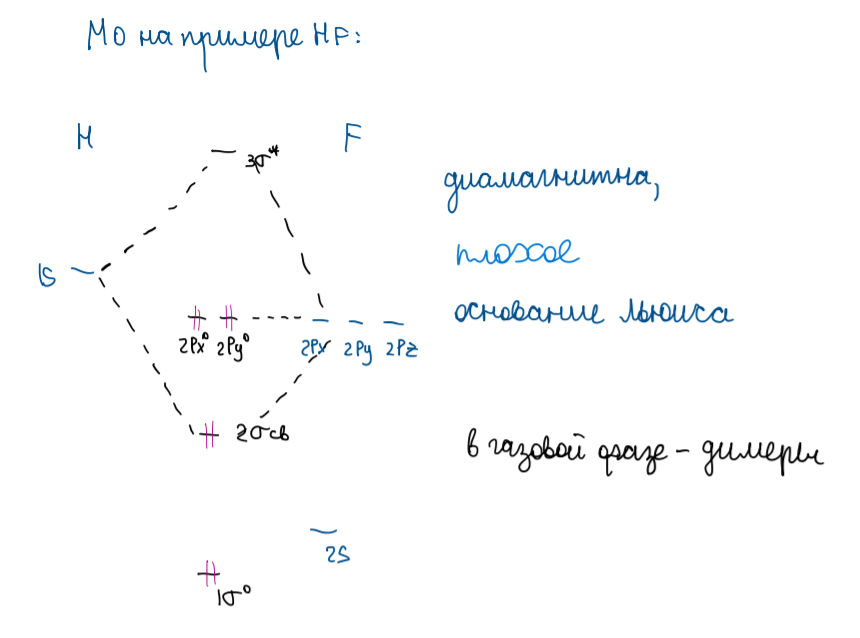
\includegraphics{4v1.png}

\subsubsection{Галогениды}

\textbf{Способы получения}

1) Обменные реакции солей

2) Металлы (до Сг) c HX

$$Me + HX \rightarrow MeX_n + H_2\uparrow$$

3) Прямое воздействие металла с $X_2$

$$2Sb + 3I_2 \rightarrow 2SbI_3 (C_6H_6)$$

4) Галогенирование оксидов с помощью $Cl_2(Br_2)$ в присутствии угля

$$Ta_2O_5 + 5C + 5Br_2 \rightarrow 2TaBr_5 +5CO \uparrow$$

(галогенирующими веществами могут быть $NH_4Cl, CCl_4, CoCl_2, ClF_3$)

5) Дегидратация кристаллогидратов

$$NiCl_2\cdot6H_2O + 6SOCl_2 \rightarrow NiCl_2 + 6SO_2\uparrow + 12HCl\uparrow$$

\textbf{{Химические свойства}}

1) Обменные реакции с солями
2) Гидролиз
$$PCl_5 + 4H_2O \rightarrow 5HCl + H_3PO_4$$
3) Восстановители

$$MeI_2 + H_2SO_{4(konc)} \rightarrow I_2 + H_2S + MeSO4 + H_2O$$
$$MeBr_2 + H_2SO_{3(konc)} \rightarrow Br_2 + SO_2 + MeSO_4 + H_2O$$

\textbf{Электронное и геометрическое строение молекул}

1) Ионные (Щ, Щ/М, РЗ металлы)

$NaCl$ - ГЦК, кч=6\\
$CsCl$ - ОЦК, кч = 8\\
$CaF_2$ - КЧ($Ca^{2+}$) =8; кч($F^-$) =4

2) Ковалентные

d-Me в низких с.о., p-Me с низкой эо.

3) Молекулярные

p-Me с высокой эо, d-Me в высших с.о.

\subsubsection{Межгалогенные соединения}

\textbf{Способы получения}

1) Непосредственное взамодействие простых веществ при варьировании соотношения реагентов, температуры и давления

2) Из сложных веществ галогенирующими агентами

$$KI + 4F_2 \rightarrow KF_{tv} + IF_7 (250^{\circ})$$

3) Галогенирование низших галогенидов

$$ClF_3 + F_2 \rightarrow ClF_5$$

\textbf{Химические свойства}

1) С $H_2O$

a) Гидролиз
$$BrF_5 + 3H_2O \rightarrow HBr_O3 + 5HF$$

б) Диспропорционирование

$$5ICl_3 + 9H_2O \rightarrow I_2 + 3HIO_3 + 15HCl$$

2) В качестве галогенирующих агентов

$$W + 6ClF \rightarrow WF_6 + 3Cl_2$$
$$2Co_3O_4 + 6ClF_3 \rightarrow 6CoF_3 + 3Cl_2 + 4O_2$$

3) Кислотно-основные свойства

$$BrF_3 + CsF \rightarrow CsBrF_4$$
$$BrF_3 + SbF_5 \rightarrow [BrF_2]^+[SbF_6]^-$$

4) С растворами щелочей до соответствующих солей: 

$$IF_5 + 6NaOH \rightarrow 5NaF + NaIO_3 + 3H_2O$$

\textbf{Электронное и геометрическое строение}

Все молекулы диамагнитны\\
Строение описывается на основе метода Гиллеспи

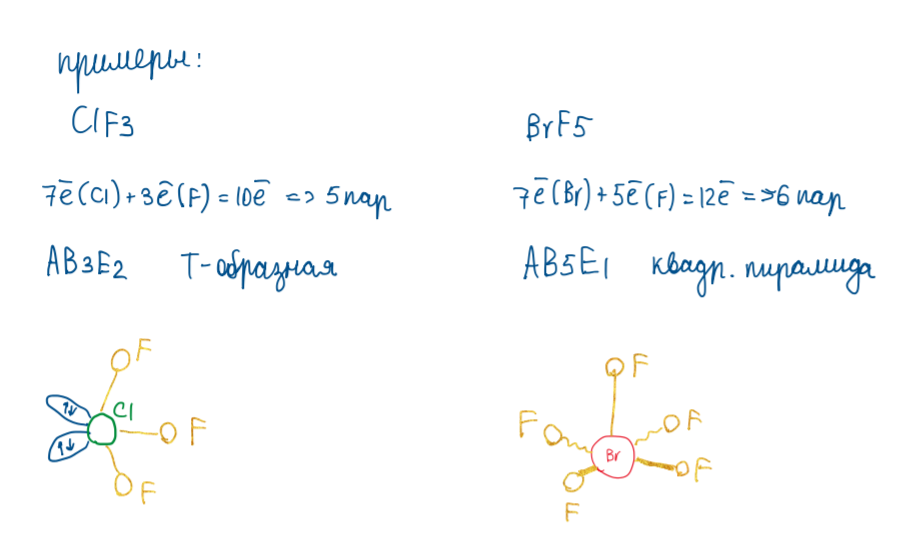
\includegraphics{4v2.png}

\subsection{Основные типы соединений галогенов в высших степенях окисления, способы получения, химическое поведение, электронное и геометрическое строение молекул.}

\subsubsection{Межгалогенные соединения}

\textbf{Способы получения}

1)Прямой синтез

$$Cl_2 + 5F_2 \rightarrow 2CiF_5 (350^{\circ}, 250 atm)$$
$$Br_2 + 5F_2 \rightarrow 2BrF_5 (>150^{\circ})$$
$$I_2 + 5F_2 \rightarrow 2IF_5 (20^{\circ})$$
$$I_2 + 7F_2 \rightarrow 2IF_7 (250-300^{\circ})$$

2) Из сложных веществ

$$MCl_{tv} + 4F_2 \rightarrow MF_{tv} + ClF_5(100-300^{\circ})$$
$$KBr + F_2 \rightarrow KF_{tv} + BrF_5$$
$$I_2 \rightarrow IF_5 (kat=AgF,ClF_3, BrF_3)$$
$$KI + 4F_2 \rightarrow KF_{tv} + 2IF_7$$
$$PdI_2 + 8F_2 \rightarrow PdF_2 + 2IF_7$$
В частности фторирование низшего фторида:
$$ClF_3 + F_2 \rightarrow ClF_5$$

\textbf{Химические свойства}

$ClF_5, BrF_5, IF_7$ - исключительно сильные фторирующие агенты, $IF_5$ - более мягкий

$$ClF_5 + 2H_2O \rightarrow ClO_2F + 4HF$$
$$ClF_5 + MeF_5 \rightarrow [ClF_4]^+[MeF_6]^-(Me= Al,Sb)$$

$$BrF_5 + 3H_2O \rightarrow HBrO_3 + 5HF (CH_3CN)$$
$$BrF_5 + CsF \rightarrow CsBrF_6\downarrow$$
$$BrF_5 + 2SbF_5 \rightarrow[BrF_4]^+[Sb2F11]^-$$
$$BrF_5 + SO_3 \rightarrow [BrF_4]^+[SO_3F]^-$$

$IF_7$ - с большинством простых веществ;

$$IF_7 + H_2O \rightarrow IOF_5 + 2HF$$
$$2IF_7 + SiO_2 \rightarrow 2IOF_5 + SiF_4 (100^{\circ})$$
$IF_5$ - донор фторид-иона($AsF_5,SbF_5$), акцептор фторид-иона ($CsF, NOF$)

$$IF_5 \rightarrow [IF_4]^+(c\ SbF_5)$$
$$IF_5 \rightarrow [IF_6]^-(c\ NOF)$$

Часто фторирование до частично фторированных аддуктов:

$$IF_5 + KMnO_4 \rightarrow MnO_3F + IOF_3 + KF$$

Образует аддукты с $XeF_2,\ XeF_4$

$$IF_5 + 3H_2O \rightarrow HIO_3 + 5HF$$
$$IF_5 + 6KOH_{aq}\rightarrow KF_{aq}+ KIO_{3(aq)} + H2O$$

С простыми веществами:

B, P, As, Sb - воспламеняются;//
Mo, W - загораются при нагревании или бурно реагируют.

\textbf{Электронное и геометрическое строение}

Определяется методом Гиллеспи:\\

$XF_5 - AB_5E$ - квадратная пирамида, где центральный атом расположен чуть ниже плоскости 4-ч атомов F в основании пирамиды. ($C_{uv}$)

$IF_7$ пентагональная бипирамида ($D_{5h}$)

$AB_7$ с небольшими искажениями.

\subsubsection{Оксиды}
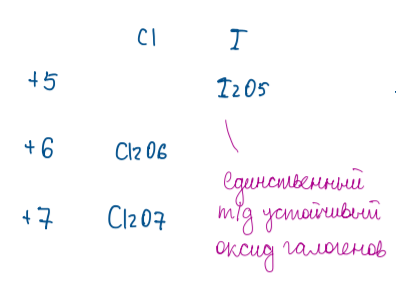
\includegraphics{5v1.png}

Br - очень неустойчивый в высших степенях окисления, немного информации о $Br_2O_5$:

Бесцветное твердое вещество, стабильно при температуре ниже $-20^{\circ}$;\\
Cтруктура $O_2Br-O-BrO_2$,  каждая $BrO_3$-группа пирамидальная с атомом $Br$  вершине.\\
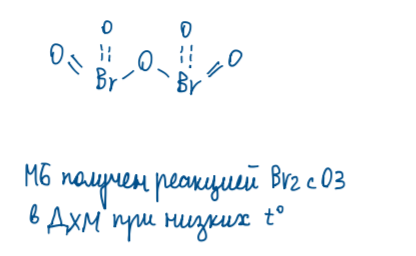
\includegraphics{5v2.png}

\textbf{Получение}

$$2ClO-2 + 2O_3 \rightarrow Cl_2O_6 + 2O_2$$
$$HClO_4 + H_3PO_4 \rightarrow Cl_2O_7 + HPO_3/(-10^{\circ})$$
$$HIO_3 \rightarrow I_2O_5 + H_2O$$
($I_2O_5$ можно получить разложением неустойчивых $I_4O_9,I_2O_4$ или $I_2 + O_2$(тлеющий разряд))

\textbf{Химические свойства}

$$Cl_2O_6 + H_2O \rightarrow HClO_3 + HClO_4$$
$$Cl_2O_6 + HF_{bezvodn}\leftrightarrow FClO_2 + HClO_4$$
$$Cl_2O_6 + Cr_2O_3/NO_xCl/NO_x \rightarrow [ClO_4]^-(x=1,2)$$
$$ Cl_2O_6 \rightarrow ClO_2 + O_2(0-10^{\circ})$$

$$Cl_2O_7 \rightarrow Cl_2 + O_2(60-70^{\circ})$$
$$Cl_2O7 +H_2O \rightarrow HClO_4$$
$$Cl_2O_7 + NaOH \rightarrow NaClO_4 + H_2O$$

$$I_2O_5 \rightarrow I_2 + O_2 (350^{\circ})$$
$$I_2O_5 + 5CO \rightarrow I_2 + 5CO_2$$
$$I_2O5 + H_2O \rightarrow HIO_3$$

\textbf{Электронное и геометрическое строение}

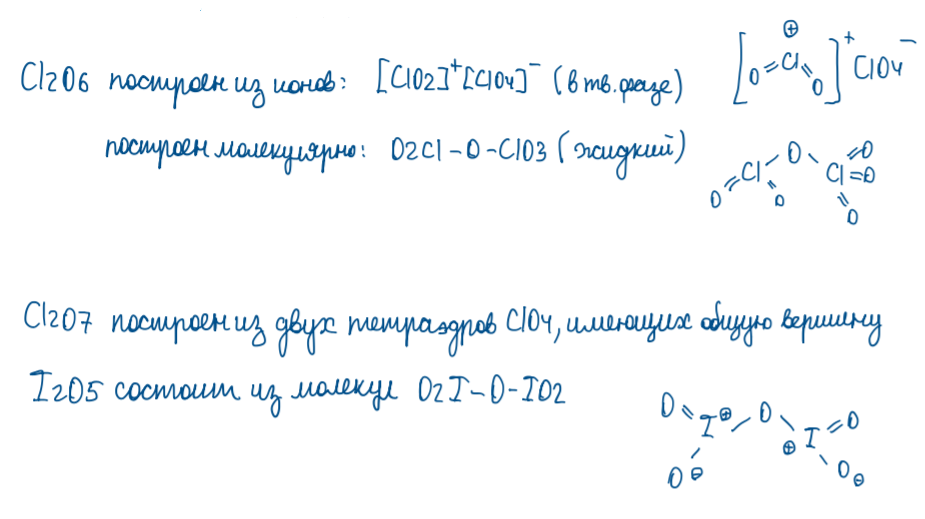
\includegraphics[scale=0.9]{5v3.png}

\subsubsection{Оксокислоты и их соли}

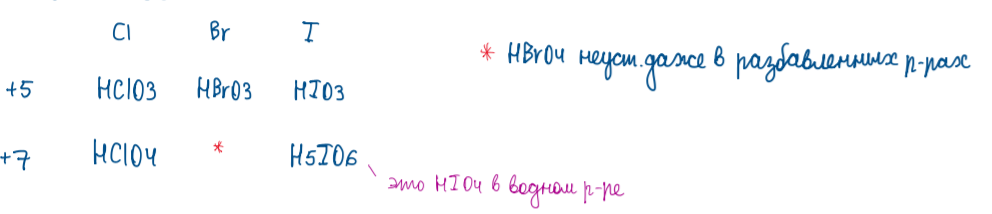
\includegraphics{5v4.png}

\textbf{Получение}

$$Ba(ClO_3)_2 + H_2SO_{4(razb)} \rightarrow HClO_3 + BaSO_4\downarrow$$
$$ I_2  + H_2O_2 \rightarrow HIO_3 + H_2O$$
$$I_2 + HNO3 \rightarrow HIO_3 + NO_2 + H_2O$$
$$I_2O_5 + H_2O \rightarrow HIO_3$$
$$HCl_{konc} + NaClO_{4(bezvodn)} \rightarrow HClO_4 + NaCl$$
$$Ba_3(H_2IO_6)_2 + HNO_3 \rightarrow H_5IO_6 + Ba(NO_3)_2$$
$$3KClO \rightarrow KClO_3 + 2KCl$$
$$KOH + X_2 \rightarrow KXO_3 + KX + H_2O$$
$$KXO_3 + I_2 \rightarrow KIO_3 + X_2$$
$$KClO_3\rightarrow 3KClO_4 + KCl (500^{\circ})$$
$$NaBrO_3 + F_2 + NaOH \rightarrow NaBrO_4 + NaF + H_2O$$
$$KOH + H_2O +KIO_3 + KClO \rightarrow K_2H_3IO_6 + KCl$$
$$K_2H_3IO_6 + HNO_3 \rightarrow KIO_4 + KNO_3 + H_2O$$

В степени окисления +5 окислительная способность меняется по ряду $Cl\approx Br > I$, сила кислот падает $Cl>Br>I$.

С увеличением степени окисления увеличивается сила кислот, но уменьшается окислительная активность.

В ряду $ClO_4^-\leq BrO_4^- \leq H_2IO_6^{3-}$ растут скорости реакции окисления

\textbf{Химические свойства}

Уменьшение силы кислот:
$$HClO_4 \rightarrow HBrO_3 \rightarrow HIO_3$$

Разложение:

$$HClO_3 \rightarrow HClO_4 + Cl_2 + O_2 + H_2O$$
$$HBrO_3 \rightarrow Br_2 + O_2 + H_2O$$
$$HIO_3 \rightarrow I_2O_5 + H_2O$$

ОВР: 

$$HIO_3 + H_2O_2 \rightarrow I_2 + O_2 + H_2O$$

Степень окисления +7 - сильные окислители ($HClO_4$ только в концентрированных растворах)

$$H_5IO_6 + HCl \rightarrow HIO_3 + Cl_2 + H_2O$$
$$H_5IO_6 + K_2CO_3 \rightarrow K_2H_3IO_6 + CO_2 + H_2O$$
$$K_2H_3IO_6 + KOH \rightarrow K_3H_2IO_6 + H_2O$$

В растворе нет 5-замещенных солей

Твердые галогенаты - сильные окислители

$$S + KBrO_3 \rightarrow K_2SO_4 + Br_2 + SO_2$$
$$KXO_3 + I_2 \rightarrow KIO_3 + X_2$$
 
$KClO_3$ - бертолетова соль

$$KClO_3 \rightarrow KCl + KClO_4$$
$$KClO_3 \rightarrow KCl + O_2 (t^{\circ}, MnO_2)$$

Степень окисления +7 -- сильные окислители (но слабее, чем сами кислоты)

$$KClO_4 \rightarrow KCl + O_2 (>550^{\circ})$$

\textbf{Электронное и геометрическое строение}

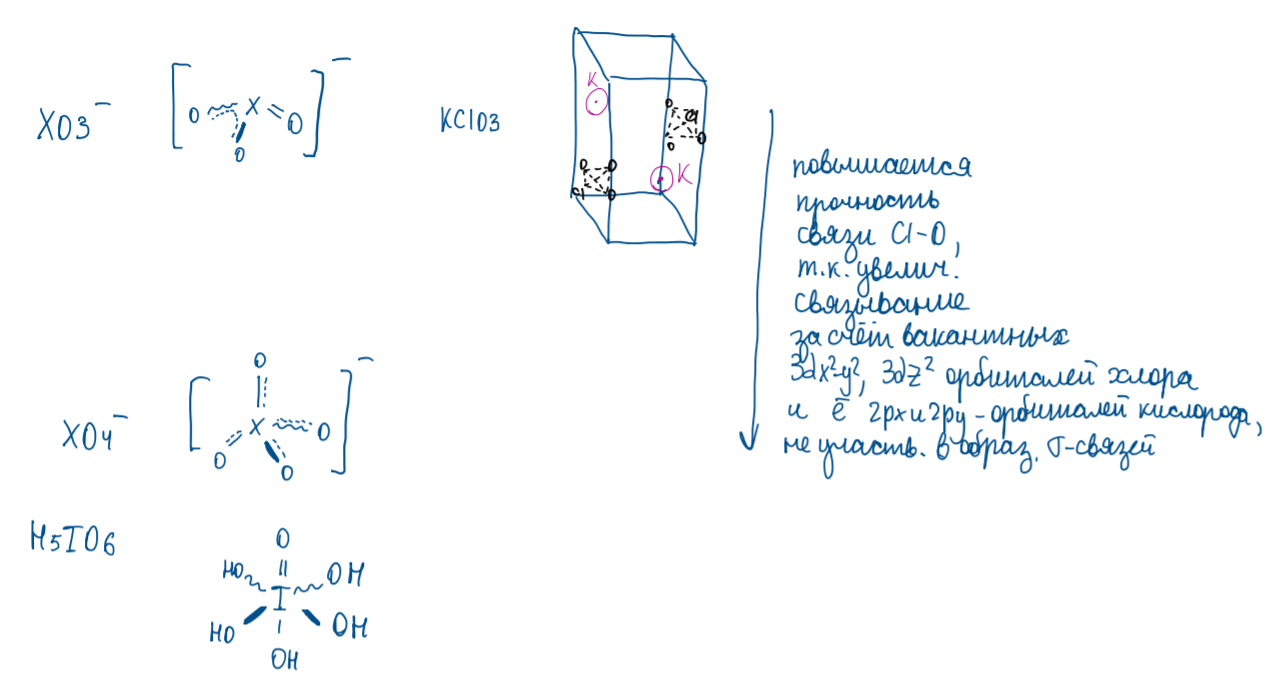
\includegraphics[scale=0.7]{5v5.png}

\subsection{Соединения кислорода и родственные им соединения серы, способы получения, химическое поведение, электронное и геометрическое строение молекул.}

\subsubsection{Кислород}

\textbf{Способы получения}
 
 Лабораторные:
 
$$H_2O_2 \rightarrow H_2O + O_2 (MnO_2)$$
$$KMnO_4 \rightarrow K_2MnO_4 + MnO_2 + O_2$$
$$KClO_3 \rightarrow KCl + O_2$$
$$KNO_3 \rightarrow KNO_2 + O_2$$

Промышленные:

Из воздуха на мембранах

$$H_2O \rightarrow H_2 + O_2$$

\textbf{Химические свойства}

1) Окисляет металлы и неметаллы (кроме легких галогенов, инертных газов и Au, Pt)

$$P_4 + O_2 \rightarrow P_2O_5$$
$$Na + O_2 \rightarrow Na_2O_2$$

2) Окисляет органические и неорганические соединения

$$E_1E_2 + O_2 \rightarrow E_{1x}O_y + E_{2z}O_{\alpha}$$
$$NeMeH + O_2 \rightarrow NeMe_xO_y + H_2O$$
$$C_xH_y + O_2 \rightarrow CO_2 + H_2O$$

3) Окисляется сильными окислителями

$$O_2 + PtF_6 \rightarrow [O_2]^+[PtF_6]$$

\textbf{Электронное и геометрическое строение}

Линейная молекула

Может быть триплетном (а) и возбужденном (б) состоянии

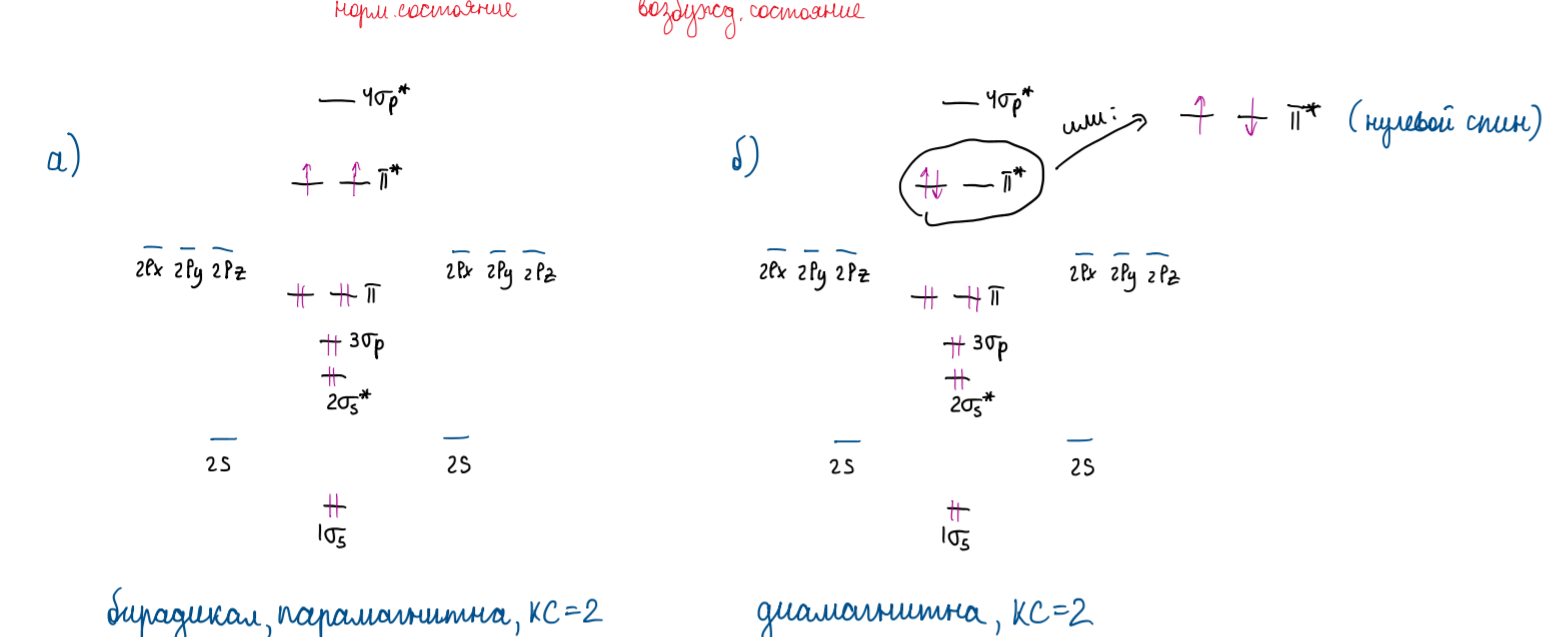
\includegraphics[scale=0.65]{6v1.png}

\subsubsection{Озон}

\textbf{Способы получения}

1) Озонирование воздуха

2) При действии тихого электрического разряда на $O_2$

$$3O_2 \rightarrow 2O_3$$

\textbf{Химические свойства}

Сильнейший окислитель (сильнее $O_2$)

$$O_3 + 2H^+ + 2e^- \rightarrow O_2 + H_2O$$
$$O_3 + H_2O + 2e \rightarrow O_2 + 2OH^-$$
$$O_3 + S + H_2O \rightarrow KOH + O_2 + I_2$$
$$O_3 + KOH \rightarrow KO_3 + O_2 + I_2$$

\textbf{Электронное и геометрическое строение}

Изогнута(угол О-О-О)= $116,8^{\circ}$

$d(O=O)_{O_2}< d(O\simeq O)_{O_3}<d(O-O)_{H_2O_2}$

Каждый атом О образует одну связь с соседним атомом р-электрона. Отслаьные р-орбитали комбнируются с образованием одной несвязывающей и одной разрыхляющей орбиталей. Количество электронов точно соответствует заселению связывающей и несвязывающей МО.

Молекула диамагнитна

\subsubsection{Сера}

Аллотропия S:

- ромбическая $S_8$ устойчивая\\
- Моноклинная $S_8$\\
- Пластическая $S_n$

\textbf{Способы получения}

Неполное сгорание $MeS$ и $H_2S$

$$MeS + O_2 \rightarrow MeO + S$$
$$H_2S + O_2 \rightarrow S + H_2O$$
$$H_2S + SO_2 \rightarrow S+ H_2O$$

\textbf{Химические свойства}

1) С простыми веществами
$$S + O_2 \rightarrow SO_2$$
$$P + S \rightarrow P_2S_3$$
$$S+F_2 \rightarrow SF_6$$
$$Me + S \rightarrow MeS$$

2) Окисление

$$S + HClO_3 + H_2O \rightarrow H_2SO_4 + HCl$$

3) Образование поликатионов

$$S_8 + AsF_5 \rightarrow [S_8]^{2+}[AsF_6]_2^- + AsF_3(SO_2 liq)$$

4) Диспропорционирование

$$S + Na_2SO_3 \rightarrow Na_2S_2O_3$$
$$S + MeOH \rightarrow MeS + MeSO_3 + H_2O$$

\textbf{Электронное и геометрическое строение}

Устойчивые гомоцепи -S-S- (зигзагообразно)\\
$S_8$ - циклическая молекула, форма короны\\
Ромбическая - форма прямоугольного параллелепипеда;\\
моноклинная - скошенный параллелепипед;\\
пластическая - скрученные спиральные цепи.

\subsubsection{Вода}

\textbf{Способы получения}


1) Продукт в огромном количестве реакции

2) Физические методы (дистилляция)

3) $H_2 + O_2 \rightarrow H_2O$

\textbf{Химические свойства}

1) Автопротолиз

$$2H_2O \leftrightarrows H_3O^+ + OH^-$$

2) Окислитель

$$H_2O + Al_{amalgama}\rightarrow Al(OH)3 + H_2$$

3) Восстановитель

$$H_2O + CoF_3 \rightarrow CoF_2 + O_2 + HF$$

\textbf{Электронное и геометрическое строение}

Угловая форма ($AB_2E_2$  по Гиллеспи)

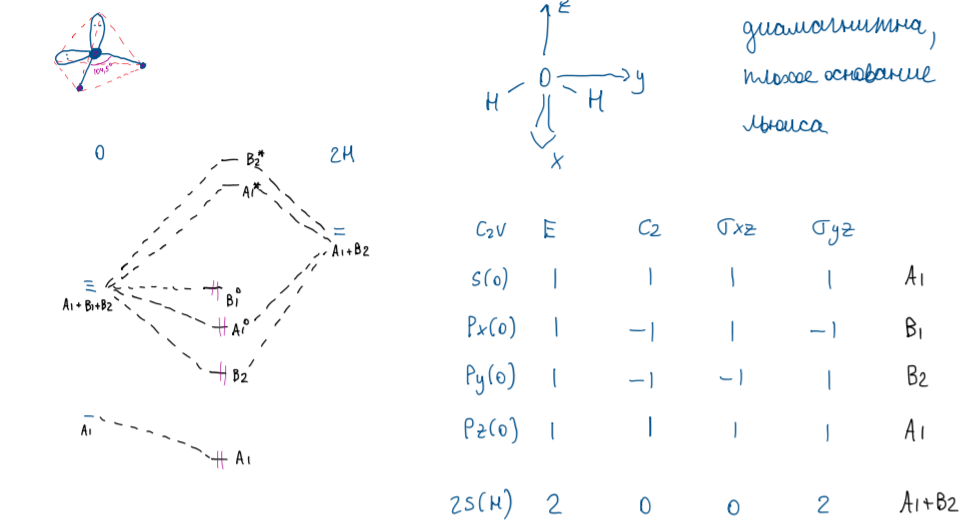
\includegraphics{6v2.png}

\subsubsection{Пероксид водорода}

\textbf{Методы получения}

$$BaO_2 + H_2SO_4 \rightarrow BaSO_4\downarrow + H_2O_2$$
$$ (CH_3)_2CHOH + O_2 \rightarrow (CH_3)_2CO + H_2O_2$$

Окисление гидроантрахинонаксилородом воздуха в органическом растворителе

\textbf{Химические свойства}

1) Разложение
$$H_2O_2 \rightarrow H_2O + O_2$$

2) Слабая кислота

$$H_2O_2 + H_2O \rightarrow H_3O^+ + HO_2^-$$
$$H_2O_2 + NaOH \rightarrow Na_2O_2 + H_2O$$

3) $Red/ox$ свойства

- сильный окислитель в кислой среде

$$NaI + H_2O_2 + H_2SO_4 \rightarrow I_2 + Na_2SO_4 + H_2O$$

- Восстановитель в кислой среде

$$KMnO_4 + H_2O_2 + H_2SO_4 \rightarrow MnSO_4 + K_2SO_4 + H_2O + O_2$$

- Окислитель в щелочной среде

$$Cr(OH)_3 + H_2O_2 + KOH \rightarrow K2CrO_4 + H_2O$$

- Восстановитель в щелочной среде

$$KOH + Cl_2 + H_2O_2 \rightarrow KCl + O_2 + H_2O$$

- Гетерогенный окислитель

$$PbS_{tv.} + H_2O_2 \rightarrow PbSO_4{tv.} + H_2O$$

\textbf{Электронное и геометрическое строение}

Строение обусловлено взаимным отталкиванием между неподеленными парами $e^-$ O и $e^-$ связи $O-H$

Молекула сильно полярна

НЭП 0 $\Rightarrow$ Д/А связи

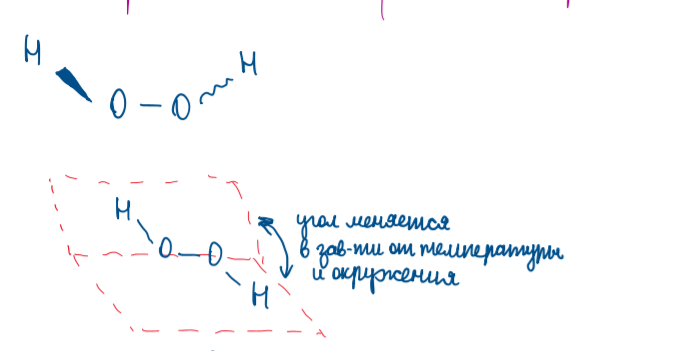
\includegraphics[scale=0.95]{6v3.png}

\subsubsection{Сероводород}

Пиросульфаны $H_2S_n$ термодинамически неуйстойчивы, например,  $H_2S_2$ разлагается водой на $S$ и $H_2S$; проявляет окислительные свойства, строение близко к $H_2O_2$

\textbf{Способы получения}

$$FeS + HCl \rightarrow FeCl_2 + H_2S$$

Гидролиз $CaS, BaS, Al_2S_3$

$$H_2 + S \rightarrow H_2S (600^{\circ})$$

\textbf{Химические свойства}

1) Слабая кислота в растворе

$$H_2S + CuSO_4 \rightarrow CuS\downarrow + H_2SO_4$$
$$NaOH + H_2S \rightarrow NaHS (Na_2S) + H_2O$$

2) Окисление

$$H_2S + I_2 \rightarrow HI + S$$
$$H_2S + SO_2 \rightarrow S+ H_2O$$
$$H_2S + H_2SO_4 + KMnO_4 \rightarrow K_2SO_4 + H_2O + S$$
$$H_2S + O_2 \rightarrow SO_2 + H_2O$$

\textbf{Электронное и геометрическое строение}

Угловая молекула, полярна\\
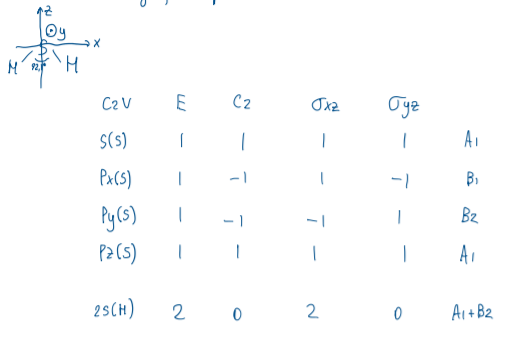
\includegraphics{6v4.png}
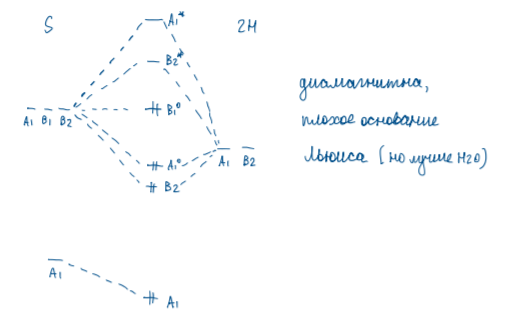
\includegraphics{6v5.png}

\subsubsection{Оксиды - большое многообразие (кислотные, основные, амфотерные)}

\textbf{Способы получения}\\
1) Взаимодействие простых веществ

2) Термическое разложение некоторых солей, кислот, оснований

$$CaCO_3 \rightarrow CaO + CO_3$$
$$Cu(OH)_2 \rightarrow CuO + H_2O$$
$$H_2CO_3 \leftrightarrows H_2O _ CO_2$$

3) Горение бинарных соединений

\textbf{Химические свойства}

1) Если элемент не в высшей степени окисления, то окисление

$$SO_3 + O_2 \rightarrow SO_3$$

2) Основные оксиды:

- с $H_2O$ (Щ и Щ/М металлы кроме Mg, Be)

- C $H^+$

- С кислотными и амфотерными оксидами

3) Амфотерные оксиды:

- С $H^+$ и $OH^-$

- С основными и кислотными оксидами

\textbf{Электронное и геометрическое строение}

Многообразие форм.

К примеру, оксиды p и d элементов в низких с.о. - полимерные структуры;\\
в высоких с.о - молекулярные структуры, часто повышенная кратность связи\\
Некоторые оксиды задают структурные типы:\\
Рутил $TiO_2$

КЧ($Ti^{4+}$)=6; КЧ = ($O^{2-}$)=3

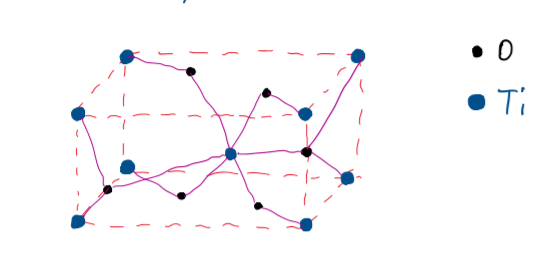
\includegraphics{6v6.png}

\subsubsection{Сульфиды}

\textbf{Способы получения}

1) Ме + S

$$Fe + S \rightarrow FeS$$
$$CdO + S \rightarrow CdS + SO_2$$
$$Ga + H_2S \rightarrow Ga_2S_3 + H_2$$

2) Обменные реакции

$$ZnCl_2 + Na_2S \rightarrow ZnS + NaCl$$

\textbf{Химические свойства}

1) Горение

$$MeS + O_2 \rightarrow MeO + S$$
$$MeS + O_2 \rightarrow MeO + SO_2$$

2) Окисление

$$CuS + HNO_{3(konc)} \rightarrow CuSO_4 + NO_2 + H_2O$$

3) Растворимые сульфиды - с солями тяжелых металлов

4) С сильными кислотами до $H_2S\uparrow$ (некоторые растворимы в кислотах : $PbS, CuS, Ag_2S, HgS, CoS, Li_2S$)

5) Необратимый гидролиз до основания и $H_2S$

\textbf{Электронное и геометрическое строение}

$M_2S$ - структура типа флюорита (каждый атом S окружен кубом из 8 атомов Me, а каждый атом Me - тетраэдром из 4 атомов S)

$MS$ -структура типа $NaCl$ (каждый атом Ме и S окружен октаэдром из атомов другого сорта)

\subsection{Соединения серы, способы получения, химическое поведение, электронное и геометрическое строение молекул.}

\subsubsection{$S_n$}

Аллотропия S:

- ромбическая $S_8$ - устойчивая\\
-моноклинная $S_8$\\
- пластическая $S_n$

\textbf{Способы получения}

1) Неполное сгорание $MeS$ и $H_2S$

$$MeS + O_2 \rightarrow MeO + S$$
$$H_2S + O_2 \rightarrow S + H_2O$$
$$H_2S + SO_2 \rightarrow S + H_2O$$

\textbf{Химические свойства}

1) С простыми веществами
$$S + O_2 \rightarrow SO_2$$
$$P + S \rightarrow P_2S_3$$
$$S+F_2 \rightarrow SF_6$$
$$Me + S \rightarrow MeS$$

2) Окисление

$$S + HClO_3 + H_2O \rightarrow H_2SO_4 + HCl$$

3) Образование поликатионов

$$S_8 + AsF_5 \rightarrow [S_8]^{2+}[AsF_6]_2^- + AsF_3(SO_2 liq)$$

4) Диспропорционирование

$$S + Na_2SO_3 \rightarrow Na_2S_2O_3$$
$$S + MeOH \rightarrow MeS + MeSO_3 + H_2O$$

\textbf{Электронное и геометрическое строение}

Устойчивые гомоцепи -S-S- (зигзагообразно)\\
$S_8$ - циклическая молекула, форма короны\\
Ромбическая - форма прямоугольного параллелепипеда;\\
моноклинная - скошенный параллелепипед;\\
пластическая - скрученные спиральные цепи.

\subsubsection{$SO_2$}

\textbf{Способы получения}

$$S + O_2 \rightarrow SO_2$$
$$FeS + O_2 \rightarrow Fe_2O_3 + SO_2$$

\textbf{Химические свойства}

1) Высокая растворимость (40л $SO_2$ ы 1 л $H_2O$)
$$SO_2 + H_2O \leftrightarrows H_2SO_3$$

2) Горение

$$SO_2 + O_2 \rightarrow SO_3(400^{\circ},V_2O_5)$$

3) Восстановитель в щелочной среде
$$K_2CrO_4 + SO_2 + KOH + H_2O \rightarrow Cr(OH)_3 + K_2SO_4$$

4) Восстановитель в кислой среде

$$SO_2 + I_2 + H_2O \rightarrow HI + H_2SO_4$$
$$SO_2 + KMnO_4 + H_2O \rightarrow K_2SO_4 + MnSO_4 + H_2SO_4$$

5) Слабый окислитель в кислой среде 

$$SO_2 + HCl + FeC_2 \rightarrow FeCl_3 + H_2O + S$$

\textbf{Электронное и геометрическое строение}

Молекула изоэлектронна молекуле озона и имеет угловую форму

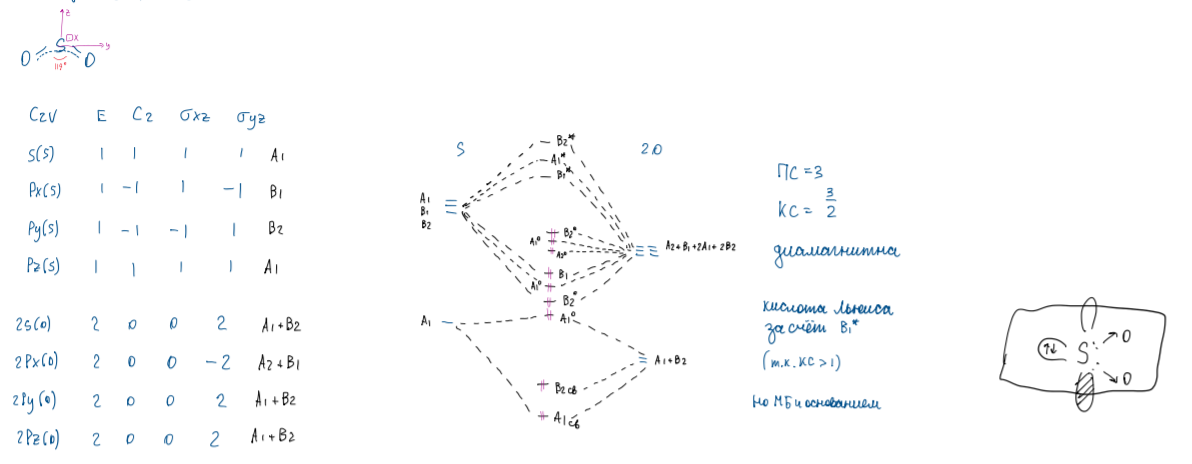
\includegraphics[scale=0.9]{7v1.png}

\subsubsection{$SO_3$}

\textbf{Способы получения}

1) Горение $SO_2$

$$SO_2 + O_2 \rightarrow SO_3 (400^{\circ})$$
2) Распад (ди-)сульфатов

$$PbSO_4 \rightarrow PbO + SO_3 (900-1100^{\circ})$$
$$BaS_2O_7 \rightarrow BaSO_4 + SO_3$$

\textbf{Химические свойства}

1) Свойства кислотного оксида:

$$SO_3 + H_2O \rightarrow H_2SO_4$$

2) Окислительные свойства 

$$SO_3 + C \rightarrow SO_2 + CO_2$$
$$SO_3 + H_2S_{gas} \rightarrow SO_2 +S + H_2O$$
$$SO_3 + F_2 \rightarrow S_2O_6F_2(170^{\circ})$$

3) Легко реагирует с донорами $e^-$

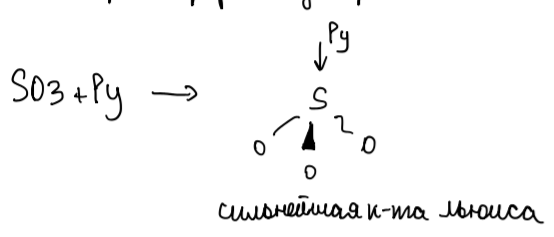
\includegraphics{7v2.png}

\textbf{Электронное строение}

Газообразное : плоский треугольник

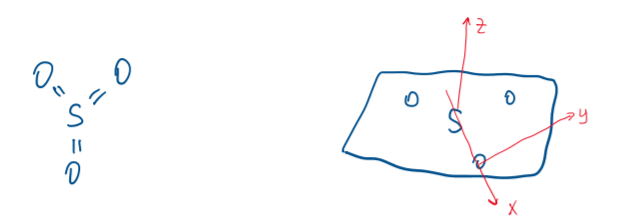
\includegraphics{7v3.png}

Кристалл - циклические тримеры $S_3O_9$ из тетраэдров $SO_4$ c общими вершинами

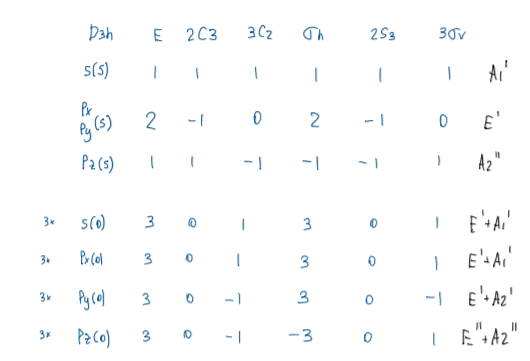
\includegraphics{7v4.png}\\
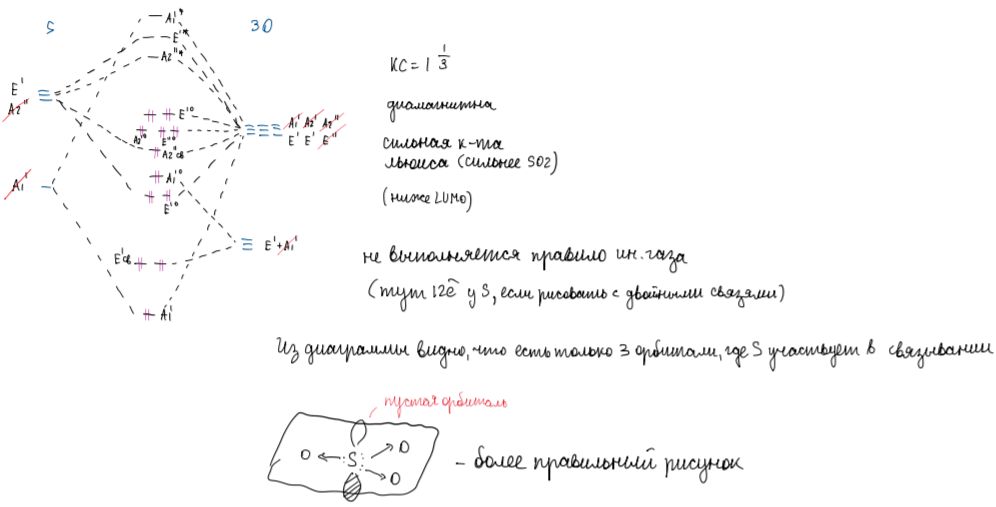
\includegraphics{7v5.png}

\subsubsection{$H_2S$}

\textbf{Способы получения}

1) Реакции обмена
$$FeS + HCl \rightarrow FeCl_2 + H_2S$$

2) Гидролиз $CaS, BaS, Al_2S_3$

3) Из простых веществ

$$H_2 + S \rightarrow H_2S(600^{\circ})$$

\textbf{Химические свойства}

1) Слабая кислота в растворе

$$H_2S + CuSO_4 \rightarrow CuS\downarrow + H_2SO_4$$
$$NaOH + H_2S \rightarrow NaHS (Na_2S) + H_2O$$

2) Окисление $$H_2S + I_2 \rightarrow HI + S$$
$$H_2S + SO_2 \rightarrow S+ H_2O$$
$$H_2S + H_2SO_4 + KMnO_4 \rightarrow K_2SO_4 + H_2O + S$$
$$H_2S + O_2 \rightarrow SO_2 + H_2O$$

\textbf{Электронное и геометрическое строение}

Угловая молекула, полярна\\
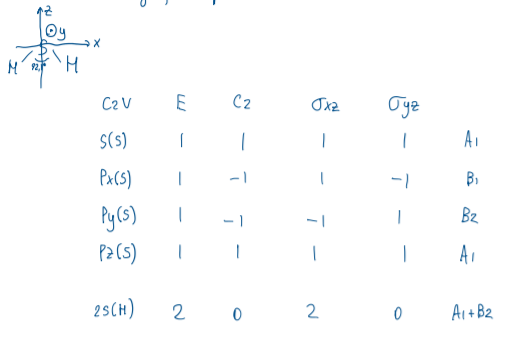
\includegraphics{6v4.png}
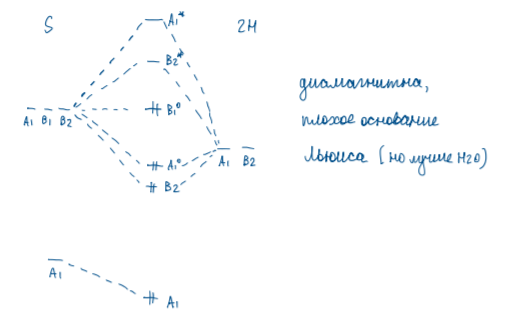
\includegraphics{6v5.png}

\subsubsection{$H_2SO_3$}

\textbf{Способы получения}

 Устойчива только в растворе, в свободном состоянии не выделена

$$SO_2 + H_2O \leftrightarrows H_2SO_3$$

\textbf{Химические свойства}

1)Диссоциация по двум ступеням

2) Мягкий восстановитель

$$Fe_2(SO_4) + SO_2 + H_2O \rightarrow FeSO_4 + H_2SO_4$$

3) Соли - восстановительные свойства

$$SO_3^{2-} + O_2 \rightarrow  SO_4^{2-}$$

4) Разложение солей

$$MeSO_3 \rightarrow MeO + SO_2 (Me = Ca, Sr, Ba)$$
$$MeSO_3 \rightarrow Me_2SO_4 + Me_2S$$

\textbf{Электронное и геометрическое строение}

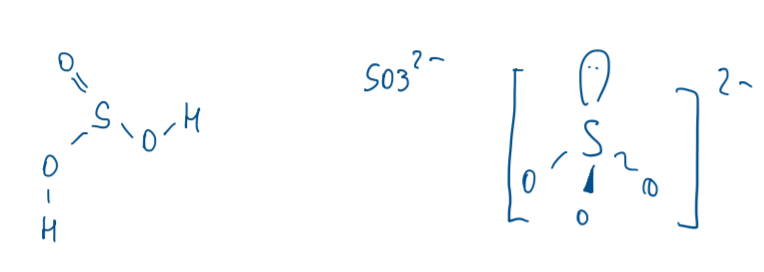
\includegraphics{7v6.png}

\subsubsection{$H_2SO_4$}

\textbf{Способы получения}

Контактный способ:

$$SO_2 + O_2 \rightarrow SO_3(400^{\circ}, V_2O_5)$$
$$SO_3 + H_2O \rightarrow H_2SO_4$$
$$H_2SO_4 + SO_3 \rightarrow H_2SO_4\cdot SO_3$$
$$H_2SO_4\cdot SO_3 +H_2O \rightarrow H_2SO_4$$

\textbf{Химические свойства}

1) Сильная кислота

$$H_2SO_4 + H_2O \rightarrow H_3O^+ + HSO_4^-$$
$$HSO_4^- + H_2O \rightarrow H_3O^+ + SO_4^{2-}$$

2) Окислитель при $\omega > 70\%$

$$Zn + H_2SO_{4(konc)} \rightarrow ZnSO_4 + SO_2 + H_2O$$
$Fe,Cr, Al$ - при нагревании

3) Водоотнонимающее средство

$$KMnO_4 + H_2SO_4 \rightarrow Mn_2O_7 + KHSO_4 + H_2O$$

4) Соли обычно растворимы (кроме $Ba, Sr, Ca$)

$$CdSO_4 \rightarrow CdO + SO_3 (1400K)$$
$$Ag_2SO_4 \rightarrow Ag + SO_2 + O_2 (1050K)$$

\textbf{Электронное и геометрическое строение}

Тетраэдрическое окружение серы

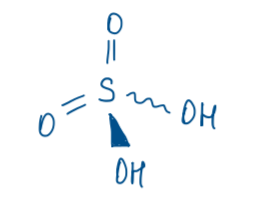
\includegraphics{7v7.png}


\subsubsection{$H_2S_2O_3$ - тиосерная, $H_2S_2O_4$ - дитионистая .... $H_2S_nO_6$ - ди-,три-, политионовая}


\textbf{Способы получения}

Обычно кислоты не стойкие, существуют только в растворах

$$HSO_3Cl + H_2S \rightarrow H_2S_2O_3 + HCl$$
$$BaS_2O_4 + H_2SO_4 \rightarrow BaSO_4\downarrow + H_2S_2O_4$$
$$BaS_2O_6 + H_2SO_4 \rightarrow BaSO_4\downarrow + H_2S_3O_6$$

$$SO_2 + H_2S + NaOH \rightarrow Na_2S_2O_3 + H_2O$$
$$Na_2SO_3 + S \rightarrow Na_2S_2O_3$$
$$Zn + SO_2 \rightarrow ZnS_2O_4$$
$$MeO_2 + 2SO_2 \rightarrow Me_2S_2O_6 (Me= Mn, Ba)$$
$$Na_2S_2O_3 +I_2 \rightarrow Na_2S_4O_6 + NaI$$

\textbf{Химические свойства}

$$H_2S_2O_3 \rightarrow H_2O + SO_2 + S$$ 

Дитионаты - устойчивы, мягкие восстановители

$$Na_2S_2O_3 + I_2 \rightarrow Na_2S_4O_6 + NaI$$

Реакция лежит в основе иодометрии

Но: с сильными окислителями до $SO_4^{2-}$

$$Na_2S_2O_3 + Cl_2 + H_2O \rightarrow H_2SO_4 + NaCl + HCl$$

Комплексообразователи:

$$Na_2S_2O_4 + Fe_2(SO_4)_3 + H_2O \rightarrow FeSO_4 + Na_2SO_4 + H_2SO_4$$

$S_2O_6^{2-}$ - нет $red/ox$ свойств, используются, как инертные анионы.

$$BaS_2O_6 + H_2SO_4 \rightarrow BaSO_4\downarrow + H_2S_2O_6$$

Разложение:

$$H_2S_2O_6 \rightarrow H_2SO_4 + SO_2 (50^{\circ})$$
$$BaS_2O_6 \rightarrow BaSO_4 + SO_2$$

\textbf{Электронное и геометрическое строение}

Удобно рассматривать, как результат замещения $O$ или $OH^-$ на изоэлектронные частицы.

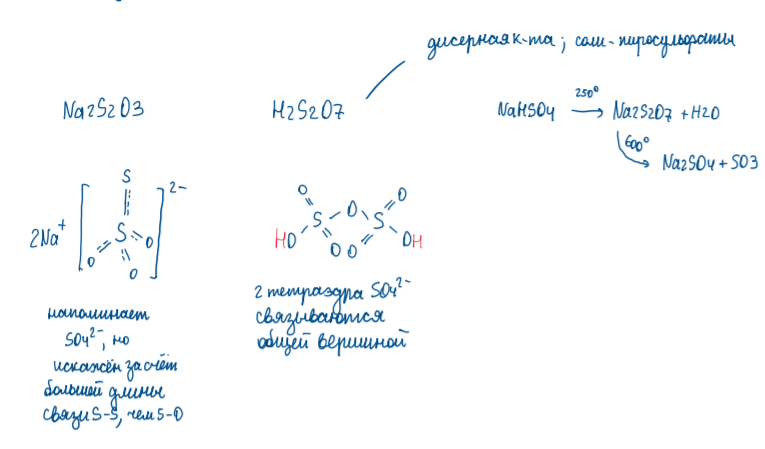
\includegraphics{7v8.png}

\subsubsection{$H_2SO_5$ - кислота Каро (пероксомоносерная)}

\textbf{Способы получения}

$$H_2S_2O_8 + H_2O \rightarrow H_2SO_4 + H_2SO_5(0^{\circ})$$
$$H_2O_2 + HSO_3Cl \rightarrow H_2SO_5 + HCl$$

\textbf{Химические свойства}

1) Окислитель

$$H_2SO_5 + H_2O \rightarrow H_2SO_4 + H_2O_2$$

\textbf{Электронное и геометрическое строение}

Образуется при замене атома $O$ у $OH-$ группы в $H_2SO_4$ на перекисную группу

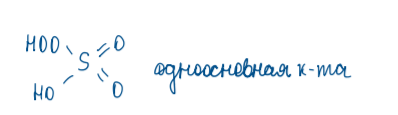
\includegraphics{7v9.png}

\subsubsection{$H_2S_2O_8$ - пероксодисерная кислота}

\textbf{Способы получения}

1) Под действием электрического тока

$$H_2SO_4 \rightarrow H_2S_2O_8 + H_2$$
$$KHSO_4 \rightarrow K_2S_2O_8 + H_2$$

\textbf{Химические свойства}

1) Сильный окислитель

$$H_2S_2O_8 + H_2O + MnSO_4 \rightarrow HMnO_4 + H_2SO_4$$

2) Используется для получения $H_2O_2$

$$H_2S_2O_8 + H_2O \rightarrow H_2SO_4 + H_2O_2 (20^{\circ})$$

\textbf{Электронное и геометрическое строение}

Образуется при замене мостикового кислорода пиросерной кислоты на перекисную группу $-O-O-$

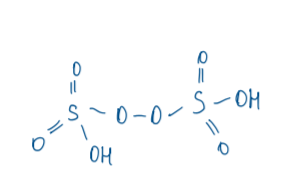
\includegraphics{7v10.png}

\subsubsection{Галоленокислоты}

$HSO_3F$ - фторсульфоновая\\
$HSO_3Cl$ - хлорсульфоновая

\textbf{Способы получения}

$$SO_{2(liq.)} + HX \rightarrow HSO_3X(X=Cl,F)$$

\textbf{Химические свойства}

1) Очень сильные кислоты

2) С $H_2O_2$

$$HSO_3Cl + H_2O_2 \rightarrow H_2SO_5 + HCl$$

3) С $H_2S$ (до $HCl, H_2S_2O_3$ при $t<0^{\circ}$) 


\textbf{Электронное и геометрическое строение}

Получаются замещением $OH-$группы серной кислоты на изоэлектронные группы $Cl^-, F^-$

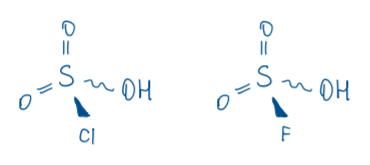
\includegraphics{7v11.png}

\subsection{Соединения азота, способы получения, химическое поведение, электронное и геометрическое строение молекул.}

\subsubsection{Азот}

\textbf{Способы получения}

1) Промышленный

Фракционирование воздуха или разделение воздуха на мембранах

2) Лабораторный

$$2NaN_3 \rightarrow 2Na + 3N_2$$
$$NH_4NO_4 \rightarrow N_2 + H_2O$$
$$NH_3 + O_2 \rightarrow N_2 + H_2O$$

\textbf{Химические свойства}

Низкая реакционная способность

1) С Ме при нагревании ( с Li при н.у.)

$$3Mg + N_2 \rightarrow Mg_3N_2 (450^{\circ})$$
$$6Li + N_2 \rightarrow 2Li_3N$$

2) C $H_2$

$$N_2 + H_2 \leftrightarrows NH_3 (p,t,kat)$$

3) С $O_2$ (электрический разряд)

$$N_2 + O_2 \rightarrow 2NO$$

4) С комплексами переходных металлов

$$[Ru(NH_3)_5(H_2O)]Cl_3 + N_2 + Zn/Hg \rightarrow [Ru(NH_3)_5(N_2)]Cl_2 + ZnCl_2 + Hg + H_2O$$

\textbf{Электронное и геометрическое строение}

Линейная молекула, $\mu=0$\\
Строение молекулярное в паре, жидкости и твердой фазы\\
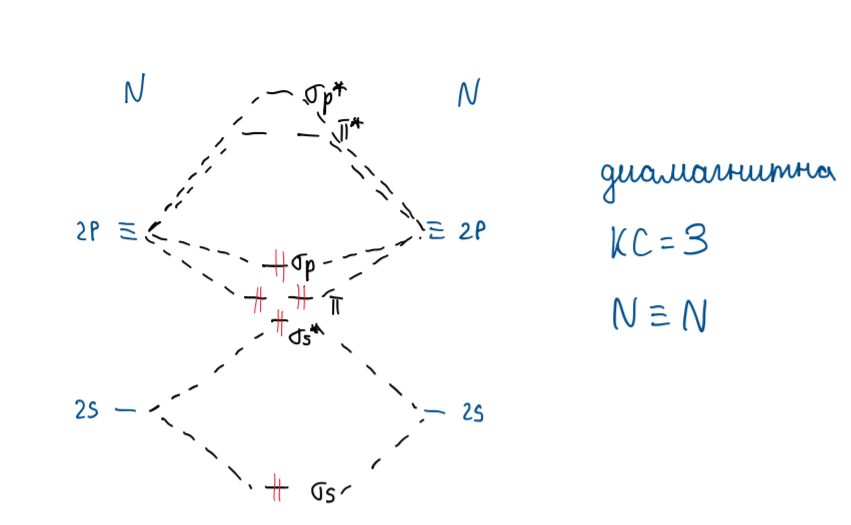
\includegraphics{8v1.png}

\subsubsection{$NH_3$}

\textbf{Способы получения}

$$Mg_3N_2 + H_2O \xrightarrow{OH^-} NH_3 + Mg(OH)_2$$
$$NH_4Cl + Ca(OH)_2 \rightarrow CaCl_2 + H_2O + NH_3$$
$$KNO_3 + Zn + KOH + H_2O \rightarrow NH_3 + K_2[Zn(OH)_4]$$

Процесс Боша-Хабера:

$$ N_2 + H_2 \leftrightarrows NH_3 (p=200 atm, \ T = 450^{\circ},\ Fe_3O_4 + Al_2O_3 + K_2O + SiO_2)$$

\textbf{Химические свойства}

1) Автоионизация

$$NH_3 \leftrightarrows NH_4^+ + NH_2^-$$

2)  Основание

$$NH_3 + H_2O \leftrightarrows NH_4^+ + OH^-$$
$$NH_3 + HR \rightarrow NH_4R \ (R - kislotn. ost)$$

3) Окисление

$$NH_3 + O_2 \xrightarrow{Rh/Pt} NO + H_2O$$
$$NH_3 + O_2 \rightarrow N_2 + H_2O$$
$$NH_3 + O_2 \xrightarrow{Rh/Pt} NH_4NO_3 + H_2O$$

4) Жидкий аммиак растворяет щелочные металлы:

$$K \xrightarrow{NH_{3(liq.)}} K_{solv}^+ + e_{solv}^+$$
$$ K + Ge \xrightarrow[en]{NH_{3(liq.)}} K_4Ge_9\cdot en$$

Соли Цинтля - сильнейшие восстановители

$$NH_3 + K \rightarrow KNH_2 + H_2$$

5) Образование комплексных соединений с солями Cu и Ag

$$Cu(NO_3)_2 + NH_3 \rightarrow [Cu(NH_3)_4](NO_3)_2$$
$$AgNO_3 + NH_3 \rightarrow [Ah(NH_3)_2]NO_3$$

\textbf{Электронное и геометрическое строение}

Пирамидальная молекула, плоская форма не существует, но можно оценить с помощью квантово-химических расчетов.

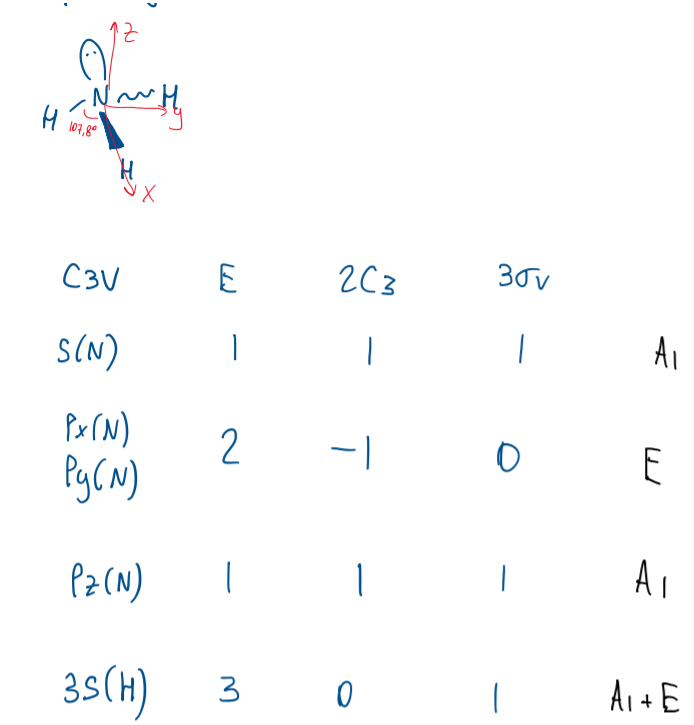
\includegraphics[scale=0.8]{8v2.png}

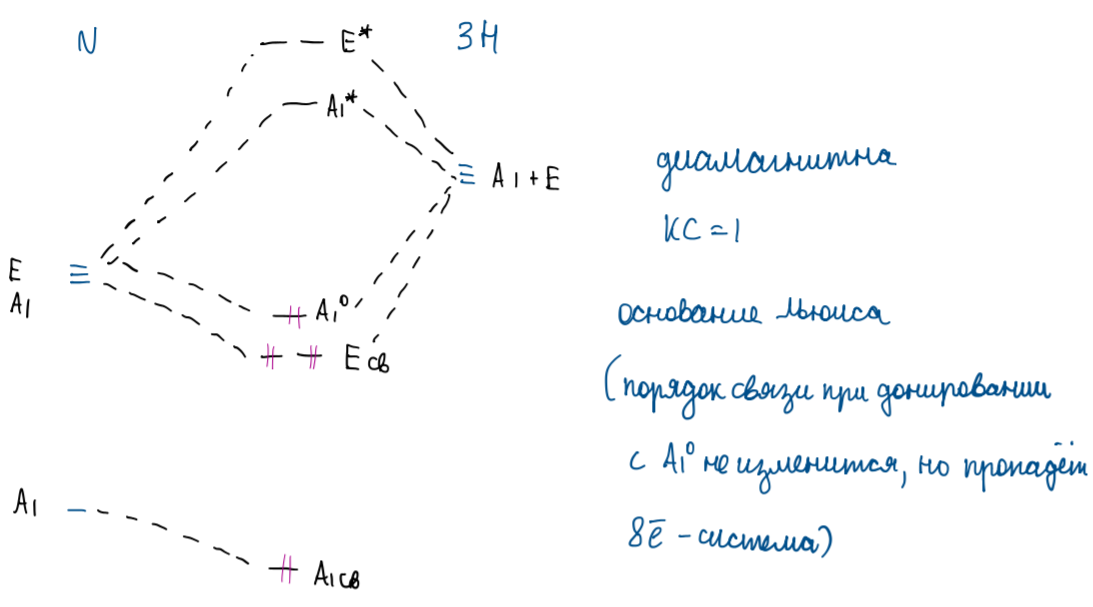
\includegraphics[scale=0.8]{8v3.png}

\subsubsection{$N_2H_4$}

\textbf{Способы получения}

$$NaClO + NH_3 \xrightarrow{Mn^{2+}} NaCl + H_2O + N_2H_4$$

\textbf{Химические свойства}

1) Основание

$$N_2H_4 + H_2O \leftrightarrows N_2H_5^+ + OH^-$$
$$N_2H_5^+ + H_2O \leftrightarrows N_2H_6^{2+} + OH^-$$

2) Окисление

$$N_2H_4 + O_2 \rightarrow N_2\uparrow + H_2O \uparrow$$

3) Разложение

$$N_2H_4 \xrightarrow{200-300^{\circ}} N_2 + NH_3$$
$$N_2H_4 \xrightarrow{Pt/Rh/Pd} N_2 + H_2$$

4) Сильный восстановитель

$$N_2H_4 + Zn + HCl \rightarrow ZnCl_2 + NH_4Cl$$
$$KMnO_4 + N_2H_4 + H_2SO_4 \rightarrow K_2SO_4 + MnSO_4 + H_2O + N_2$$

\textbf{Электронное и геометрическое строение}

Две группы $NH_2$, повернутые относительно друг друга, молекула полярная.

У атомов азота по одной НЭМ.

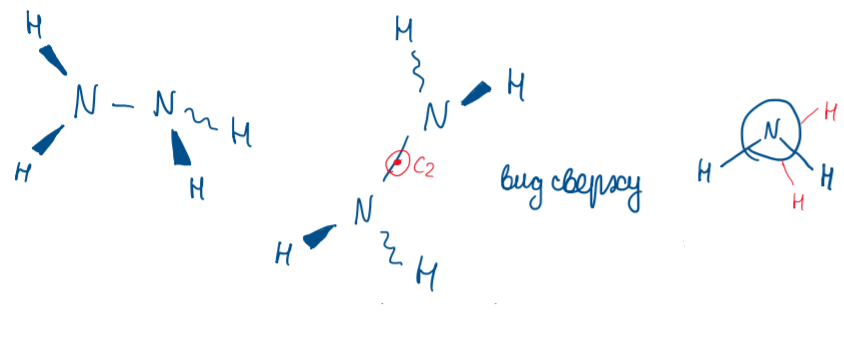
\includegraphics{8v4.png}

\subsubsection{$HN_3$}

\textbf{Способы получения}

$$NaNH_2 + N_2O \xrightarrow{200^{\circ}} NaN_3 + NaOH + NH_3$$
$$NaN_3 + H_2SO_4 \rightarrow Na_2SO_4 + NH_3$$

\textbf{Химические свойства}

1) Слабая кислота

$$HN_3 \leftrightarrows H^+ + N_3^-$$

2) Окислитель

$$Cu + HN_3 \rightarrow Cu(N_3)_2 + N_2 + NH_3$$
$$HCl + HN_3 \rightarrow NH_4Cl + Cl_2 + N_2$$

3) Разложение

$$HN_3 + H_2O \rightarrow N_2 + NH_2OH$$

4) Соли - азиды, неустойчивы и взрывчаты

Азиды щелочных металлов (не Li) и тяжелых металло при t $\rightarrow Me + N_2$
(Получение очень чистых металлов)

Азиды щелочноземельных металлов и Li разлагаются на нитрид и $N_2$\\
\\

\textbf{Электронное и геометрическое строение}

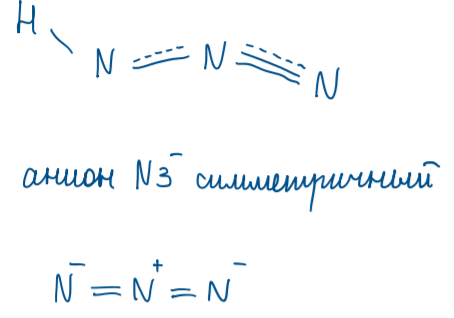
\includegraphics{8v5.png}

Можно рассмотреть как результат замены в $N_2O$ атома $O$ на группу $N-H$

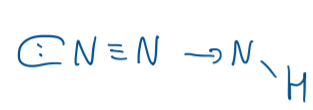
\includegraphics{8v6.png}

\subsubsection{$N_2O$}

\textbf{Получение}

$$NH_4NO_3 \xrightarrow{250^{\circ}} N_2O + H_2O$$
$$NH_2OH + HNO_2 \rightarrow N_2O + H_2O$$

\textbf{Химические свойства}

1) Несолеобразующий

2) Разложение

$$N_2O \xrightarrow{700^{\circ}} N_2 +O_2$$

3) Поддерживает горение

$$N_2O + H_2 \rightarrow N_2 + H_2O$$
$$N_2O + C \rightarrow N_2 + CO$$
$$N_2O + P \rightarrow N_2 + P_2O_5$$

\textbf{Электронное и геометрическое строение}

Линейная молекула, помимо $\sigma$-связей есть второстепенное взаимодействие p-орбиталей 2-типа.

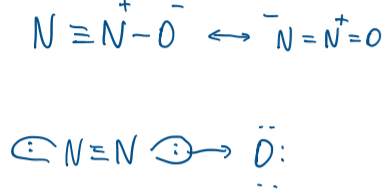
\includegraphics{8v7.png}

\subsubsection{$NO$}

\textbf{Получение}

1) Каталитическое окисление аммиака (промышленный способ)

$$NH_3 + O_2 \xrightarrow{kat, 1000^{\circ}} NO + H_2O$$
$$N_2 + O_2 \xrightarrow{2000^{\circ}} NO$$

2) В лабаратории

$$ Cu + HNO_{3(razb.)}\rightarrow Cu(NO_3)_2 + H_2O + NO$$
$$KNO_2 + KI + H_2SO_4 \rightarrow K_2SO_4 + I_2 + NO$$

3) Легко окисляется $O_2$ и $Hal_2$

$$NO + O_2 \rightarrow NO_2$$
$$NO + Cl_2 \rightarrow NOCl$$

4) Нерастворим в воде, не реагирует с $H^+$ и $OH^-$

5) Слабый окислитель

$$NO + H_2 \rightarrow N_2 + H_2O$$
$$NO + SO_2 \rightarrow N_2 + SO_3$$

6) Слабый восстановитель

$$NO + K_2Cr_2O_7 + H_2SO_4 \rightarrow HNO_3 + K_2SO_4 + Cr_2(SO_4)_3 + H_2O$$

\textbf{Электронное и геометрическое строение}

Линейная молекула-радикал, нет димеризации

$$NO^- \xleftarrow{+e} NO \xrightarrow{-e}  NO^+$$

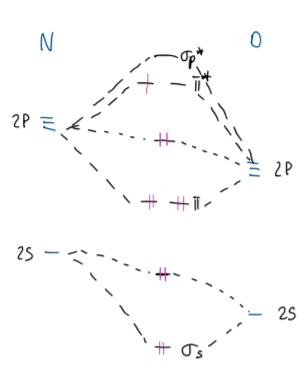
\includegraphics{8v8.png}

\subsubsection{$N_2O_3$}

\textbf{Способы получения}

$$NO_2 + NO \leftrightarrows N_2O_3$$

\textbf{Химические свойства}

1) Неусточив разлагается на $NO$ и $NO_2$

2) Ангидрид азотистой кислоты $HNO_2 \Rightarrow$ все свойства кислотных оксидов

\textbf{Электронное и геометрическое строение}

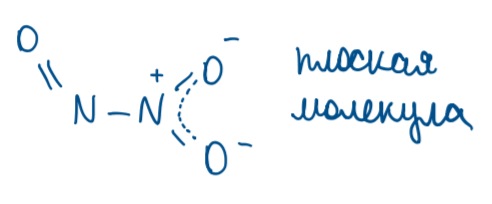
\includegraphics{8v9.png}

\subsubsection{$NO_2$}

\textbf{Способы получения}

$$NO + O_2 \rightarrow Cu(NO_3)_2 + NO_2 + H_2O$$
$$Cu + HNO_{3(konc)} \rightarrow Cu(NO_3)_2 + NO_2 + H_2O$$

Разложение нитратов:

$$Cu(NO_3)_2 \rightarrow CuO + NO_2 + O_2$$

\textbf{Химические свойства}

1) С $H_2O$

$$NO_2 + H_2O \rightarrow HNO_2 + HNO_3$$
$$NO_2 + H_2O + O_2 \rightarrow HNO_3$$

2) С щелочами

$$NO_2 + NaOH \rightarrow NaNO_2 + NaNO_3 + H_2O$$

3) Окислитель

$$NO_2 + SO_2 \rightarrow NO + SO_3$$
$$NO_2 + C \rightarrow CO_2 + N_2$$
$$NO_2 + P \rightarrow P_2O_5 + NO$$

4) Димеризация

$$2NO_2 \leftrightarrows N_2O_4$$

\textbf{Электронное и геометрическое строение}

У $NO_2$ 1 неспаренный электрон на связывающей орбитали $\Rightarrow$ выгодна димеризация

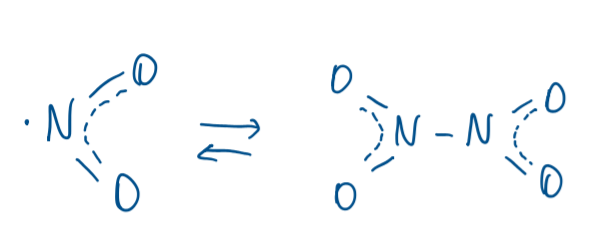
\includegraphics{8v10.png}

\subsubsection{$N_2O_5$}

\textbf{Способы получения}

$$NO_2 +O_3 \rightarrow N_2O_5 + O_2$$
$$HNO_3  + P_2O_5 \rightarrow HPO_3 + N_2O_5$$

\textbf{Химические свойства}

1) Ангидрит азотной кислоты $HNO_3 \Rightarrow$ все свойства кислотных оксидов

2) Сильный окислитель

$$N_2O_5 + I_2 \rightarrow I_2O_5 + N_2$$

3) Легко разлагается ( при нагревании со взрывом)

$$N_2O_5 \rightarrow NO_2 + O_2$$

\textbf{Электронное и геометрическое строение}

Не все атомы в одной плоскости

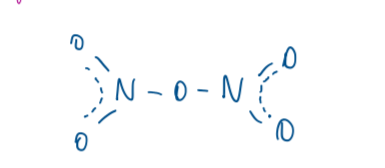
\includegraphics{8v11.png}

\subsubsection{$H_2N_2O_2$ - азотноватистая кислота}

\textbf{Способы получения}

$$Ag_2N_2O_2 + HCl \xrightarrow[-AgCl]{efir} H_2N_2O_2$$

\textbf{Химические свойства}

1) Слабая неустойчивая кислота

$$H_2N_2O_2 \xrightarrow{t} N_2O \uparrow + H_2O$$

2) Горение

$$H_2N_2O_2 +O_2 \rightarrow HNO_2 + HNO_3$$

3) Образует комплексы в d-металлами

\textbf{Электронное и геометрическое строение}

Плоская молекула

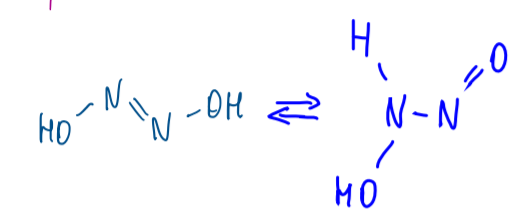
\includegraphics{8v12.png}

\subsubsection{$HNO_2$-азотистая}

\textbf{Способы получения}

$$Ba(NO_2)_2 + H_2SO_4 \rightarrow BaSO_4\downarrow + HNO_2$$
$$N_2O_3 + H_2O \rightarrow HNO_3$$

\textbf{Химические свойства}

1) Разложение

$$HNO_2 \xrightarrow{>100^{\circ}} NO + HNO_3 + H_2O$$

2) ОВР

$$HNO_2 + Br_2 + H_2O \rightarrow HBr + HNO_3$$
$$HNO_2 + FeCl_2 + HCl \rightarrow FeCl_3 + NO + H_2O$$

\textbf{Строение}

Плоская молекула

\subsubsection{$HNO_3$ - азотная кислота}

\textbf{Способы получения}

$$NH_3 + O_2 \xrightarrow{p,t,kat} NO + H_2O$$
$$NO + O_2 \rightarrow NO_2$$
$$NO_2+H_2O \rightarrow HNO_3 + HNO_2$$
$$HNO_3 \xrightarrow{t} NO + HNO_3 + H_2O$$

\textbf{Химические свойства}

1) Сильная кислота

2) Разложение при н.у (б/в)

$$HNO_3 \rightarrow NO_2 + O_2 + H_2O$$

3) Со многими металлами $H_2$ не выделяет, пассивирует $Fe,Cr,Al$

4) С неметаллами: $P, S, I,...$
$$ S + HNO_3 \rightarrow H_2SO_4 + NO_2 + H_2O$$

5) Нитраты растворимы в воде, при t разлагаются

$$KNO_3 \rightarrow KNO_2 + O_2$$
$$Cd(NO_3)_2 \rightarrow CdO + NO_2 + O_2$$
$$AgNO_3 \rightarrow Ag + NO_2 + O_2$$

6) Окислители в кислой среде и расплаве

$$MnO_2 + KOH + KNO_3 \rightarrow K_2MNO_4 + KNO_2 + H_2O$$

\textbf{Строение}

Плоская молекула

\subsubsection{$NH_2OH$ - гидроксиламин}

\textbf{Способы получения}

$$6H^+ + HNO_3 + 6e^- \rightarrow NH_2OH + H_2O$$

\textbf{Химические свойства}

1) Разложение 

$$NH_2OH \rightarrow NH_3 + N_2 +H_2O$$

2) Основание 
$$NH_2OH \rightarrow H_2O \leftrightarrows NH_3OH^+ OH^-$$

3) Восстановитель (слабее $N_2H_4$)

$$NH_2OH + I_2 \rightarrow N_2 + HI + H_2O$$

4) Соль-окислитель

$$[NH_3OH]Cl + FeCl_2 + HCl \rightarrow NH_4Cl + FeCl_3 + H_2O$$

\textbf{Строение}

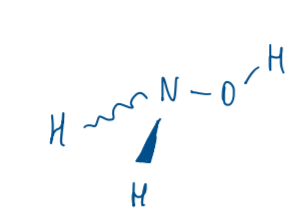
\includegraphics{8v13.png}

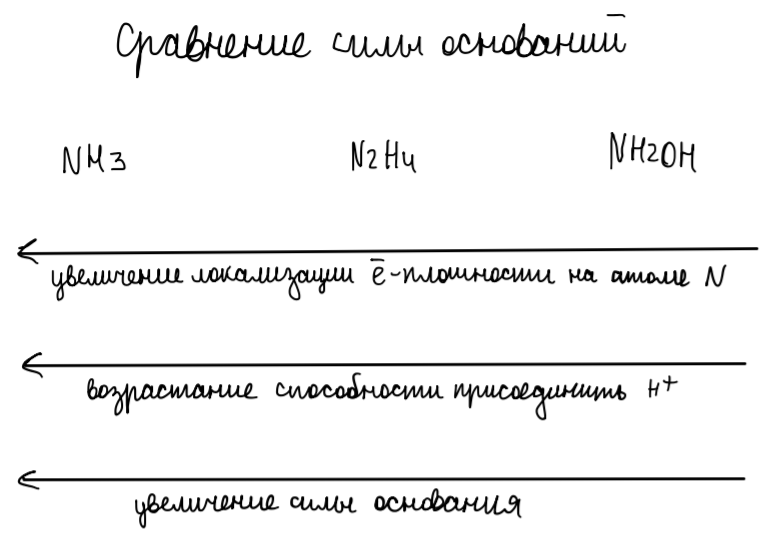
\includegraphics{8v14.png}

\subsection{Соединения фосфора, способы получения, химическое поведение, электронное и геометрическое строение молекул.}

\subsubsection{Аллотропия P}

- Белый - $P_4$ -очень реакционно способен, очень токсичный, светится в темноте\\
- Красный - P - малотоксичен, активность меньше белого\\
-Черный - химически инертный, нетоксичен

\textbf{Получение}

$$Ca3(PO_4)_2 + SiO_2 + C \xrightarrow{1400^{\circ}} CaSiO_3 + CO + P_4$$
$$HPO_3 + C \rightarrow P + H_2 + CO$$

\textbf{Химические свойства}

1) Белый фосфор - очень активный, самовоспламеняется на воздухе

$$P_4 + O_2 \rightarrow P_2O_5$$

2) Красный при $260^{\circ}$

$$P + O_2 \rightarrow P_2O_5$$

3) Черный не горит

4) $P_4 \xrightarrow{250-300^{\circ}} 4P$

5) с $H_2$ не взаимодействует

6) С водой и щелочами диспропорционирует

$$P + H_2O \rightarrow PH_3 + H_3PO_2$$
$$P + KOH + H_2O \rightarrow PH_3 + KH_2PO_2$$

7) С неметаллами и сильными окислителями - восстановитель

$$P + S \rightarrow P_2S_3$$
$$2P + 5Cl_2 \rightarrow 2PCl_5$$
$$2P + 2Cl_2 \rightarrow 2PCl_3$$

$$P + HNO_{2(konc)} \rightarrow H_2PO_4 + NO_2 + H_2O$$
$$P + H_2SO_{4(konc)} \rightarrow H_3PO_4 + SO_2 + H_2O$$
$$P + KClO_3 \rightarrow P_2O_5 + KCl$$

8) С металлами - оксилитель

$$P + Ca \rightarrow Ca_3P_2$$
\\

\textbf{Строение}

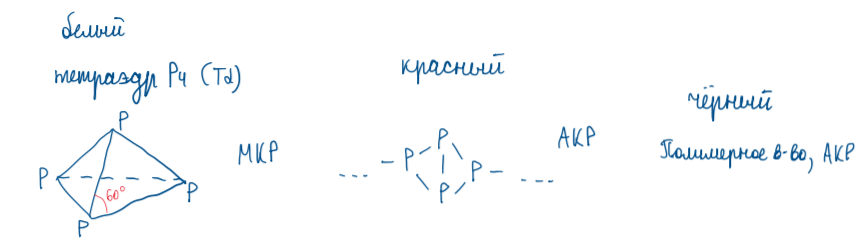
\includegraphics{9v1.png}

\subsubsection{$PH_3$ и фосфиды}

\textbf{Получение}

$$MeP + H2O \rightarrow Me(OH)_x + PH_3$$
$$P + MeOH + H_2O \rightarrow PH_3 + MeH_2PO_2$$
$$[PH_4]R + MeOH \rightarrow MeR + PH_3 + H_2O$$
$$Me + P \rightarrow MeP^{3-}$$

\textbf{Химические свойства}

1) Разложение

$$PH_3 \rightarrow P + H_2$$

2) Слабые основные свойства

$$PH_3 + HI \rightarrow [PH_4]^+I^-$$

3) Сильный восстановитель

$$PH_3 + O_2 \rightarrow HPO_3 + H_2O$$
$$PH_3 + MnO_4 + H^+ \rightarrow PO_4^{3-}+...$$

4) Фосфиды  гидролиз  и горение

$$MeP + O_2 \rightarrow MeO + P_2O_5$$
$$MeP + H2O \rightarrow Me(OH)_x + PH_3$$

\textbf{Строение}

Слабее поляризованы связи $P-H$, чем у $NH_3 \Rightarrow$ слабее как основание;\\
Активность НЭП $P (3s^2)$ ниже НЭП $N (2s^2)$, нет водородных связей

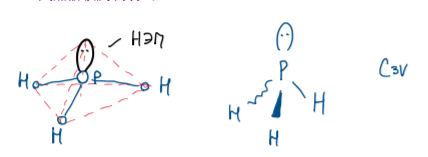
\includegraphics{9v2.png}

\subsubsection{Галогениды}

Есть в +3, и в +5, кроме $PI_5$

\textbf{Получение}

1) Прямым синтезом из простых веществ при разных условиях и соотношениях

$$2P + 5Cl_2 \rightarrow 2PCl_5$$
$$2P + 2Cl_2 \rightarrow 2PCl_3$$

$$PCl_x \xrightarrow{CaF_2/ZnF_2/AsF_3} PF_x(x=3,5)$$

\textbf{Химические свойства}

1) $PF_3$ - яд, не взаимодействует с $H_2O$, прочные комплексы с d-металлами

2) $PX_3$ - гигроскопичны (x = Cl, Br, I)

$$PX_3 + H_2O \rightarrow H_3PO_3 + HX$$

3) $PX_3$ - донорные свойства (x=Cl,Br,I)

4) $PX_5$ - галогенангидриды

$$PX_5 + H_2O \rightarrow H_3PO_4 + HX$$
$$POCl_3 + H_2O \rightarrow H_3PO_4 + HCl$$

5) Донорные свойства

$$PCl_5 + BCl_3 \rightarrow [PCl_4]^+[BCl_4]^-$$
$$PCl_5 + KF \xrightarrow{\approx 200^{\circ}} K[PF_6] + KCl$$
$$PCl_5 + NH_4Cl \rightarrow (PNCl_2)_3$$
$$PCl_5 + P_3O_10 \xrightarrow{150^{\circ}} POCl_3$$

6) С органическими веществами

$$PCl_5 + RCOOH \xrightarrow{60^{\circ}} RCOCl + POCl_3 + H_2O$$
$$PCl_5 + ROH \rightarrow RCl + POCl_3 + HCl$$

\textbf{Электронное и геометрическое строение}

$PF_5$ - молекулярный\\
$PCl_5$ - молекулярный в газовой фазе, в твердой фазе $[PCl_4]^{+}[PCl_6]^-$\\
$PBr_5$ в твердой фазе $[PBr_4][Br]^-$

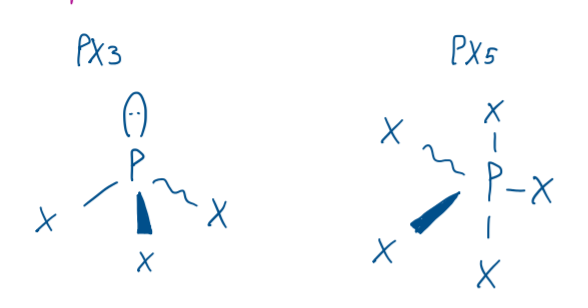
\includegraphics{9v3.png}

Диаграмма МО на примере $PF_5$ (рассматриваем p-орбитали F, направленные к P)

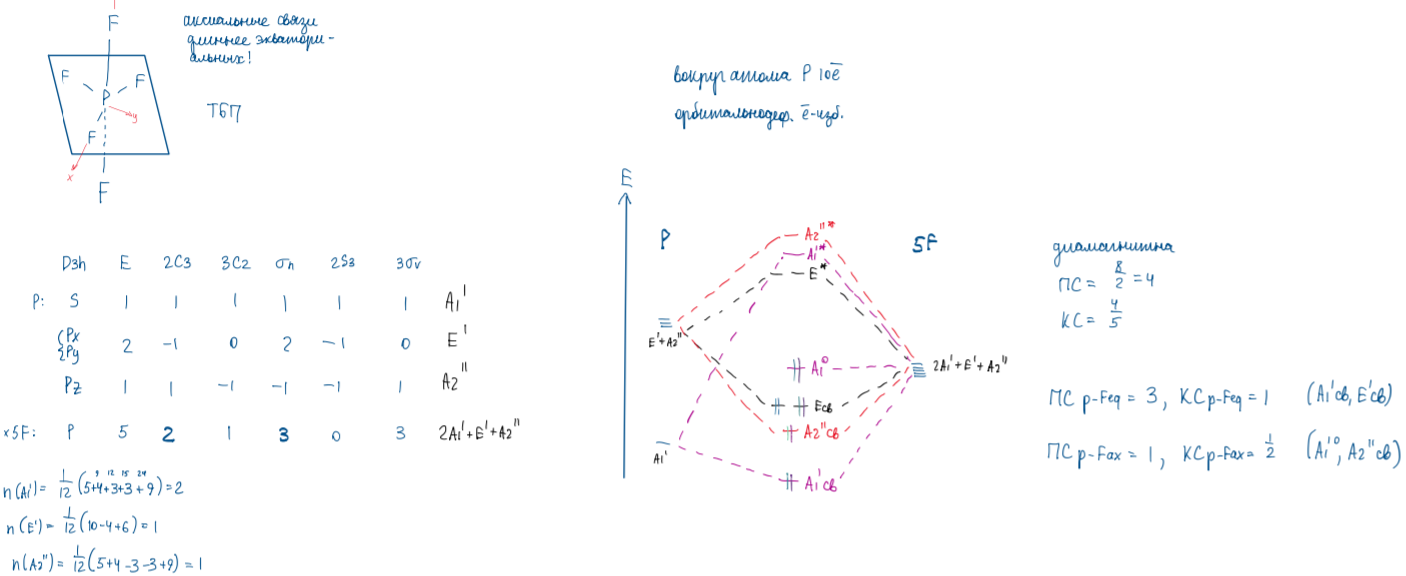
\includegraphics[scale=0.75]{9v4.png}

Аксиальные связи менее прочные и более длинные

\subsubsection{$P_2O_3 \leftrightarrow P_4O_6$}

\textbf{Получение}

$$P + O_2 \rightarrow P_2O_3$$
$$P_4 + N_2O \xrightarrow{550-635^{\circ}} P_4O_6 + N_2$$
$$P_4 + CO_2 \xrightarrow{650^{\circ}} P_4O_6 + CO$$
$$P_4 + P_4O_{10} \xrightarrow{50^{\circ}}$$

\textbf{Химические свойства}

1) Ангидрид фосфористой кислоты

$$P_4O_6 + H_2O \xrightarrow{holod} H_3PO_3$$
$$P_4O_6 + H_2O \xrightarrow{gor} P\downarrow + H_3PO_4 + PH_3\uparrow$$

2) Сильный восстановитель

$$P_4O_6 + O_2 \xrightarrow{50-120^{\circ}} P_4O_10$$
$$P_4O_6 + Cl_2  \rightarrow POCl_3 + O_2$$
$$P_4O_6 + S \rightarrow P_4S_6 + SO_2$$

\textbf{Строение}

В парах состоит из молекул $P_4O_6$\\
Тетраэдр из P, и на каждом ребре O

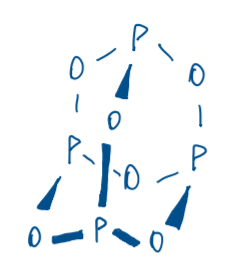
\includegraphics{9v5.png}

\subsubsection{$P_2O_5 \leftrightarrow P_4O_{10}$}

\textbf{Получение}

$$ P + O_2 \rightarrow P_4O_{10}$$

Разложение при сильном нагревании:

$$P_4O_{10} \rightarrow P_4O_6 + O_2$$

Ангидрид фосфорной кислоты

$$P_4O_{10} + H_2O \rightarrow H_3PO_4$$

Все свойства кислотных оксидов

Сильное водоотнимающее средство 

$$P_4O_{10} + HNO_3 \rightarrow HPO_3 + N_2O_5$$
$$P_4O_{10} + HClO_4 \rightarrow HPO_3 + Cl_2O_7$$

С RCOOH

$$P_4O_{10} + RCOOH \rightarrow H_3PO_4 + (RCO)_2O$$

\textbf{Строение}

В парах состоит из молекул $P_4O_{10}$\\
Кристаллическое состояние - две метастабильные модификации:

- Гексагональная н-форма ($P_4O_{10}$ 4 группы в виде тетраэдра)

-Орторомбическая о-форма (химически менее активны, полимерные структуры из тетраэдров $PO_4$)

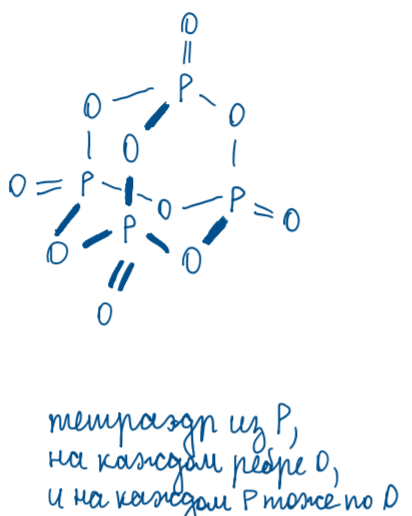
\includegraphics{9v6.png}

\subsubsection{$HPF_6$}

\textbf{Получение}

$$H_3PO_4 + HF_{konc} \rightarrow HPF_6 + H_2O$$

\textbf{Химические свойства}

1) Существуют только в растворе

$$HPF_6 \leftrightarrows H^+ + PF_6^-$$

2) Не окислитель, не коррдинирующий ион

3) Соли растворимы в воде

\textbf{Строение}

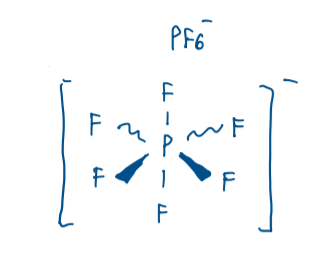
\includegraphics{9v7.png}

\subsubsection{$H_3PO_2$ - фосфорноватистая}

\textbf{Получение}

$$Ba(H_2PO_2)_2 + H_2SO_4 \rightarrow H_3PO_2 + BaSO_4 \downarrow$$

\textbf{Химические свойства}

1) Сильная одноосновная кислота

$$H_3PO_2 \leftrightarrows H^+ + H_2PO_2^-$$

2) Диспропорционирование 

$$H_3PO_2 \rightarrow PH_3 + H_3PO_4$$

3) Очень сильный окислитель

$$H_3PO_2 + FeCl_3 + H_2O \rightarrow H_3PO_4 + FeCl_2 + HCl$$
$$NaH_2PO_2 + AgNO_3 + H_2O \rightarrow NaNO_3 + Ag + H_3PO-4 + HNO_3$$
4) Соли - гипофосфиты, хорошо растворимы в воде

\textbf{Строение}

$H(PH_2O_2)$
\includegraphics{9v8.png}

\subsubsection{$H_3PO_3$ - фосфористая}

\textbf{Получение}

$$PCl_3 + H_2O \rightarrow H_3PO_3 + HCl$$
$$P_2O_3 + H_2O \rightarrow H_3PO_3$$
$$K_2HPO_3 + HCl \rightarrow KCl + H_3PO_3$$

\textbf{Химические свойства}

1) Двухосновная кислота средней силы, соли фосфины

2) Диспропорционирование

$$H_3PO_3 \rightarrow PH_3 + H_3PO_4$$
$$H_3PO_3 + O_2 \rightarrow H_4P_2O_6 + H_2O$$

3) Восстановительные свойства

$$H_3PO_3 + HgCl_2 + H_2O \rightarrow H_3PO_4 + Hg + HCl$$
\\
\textbf{Строение}

$H_2(PHO_3)$
\includegraphics{9v9.png}

\subsubsection{$H_4P_2O_6$ - фосфорноватая}

\textbf{Получение}

$$H_3PO_3 + O_2 \rightarrow H_4P_2O_6 + H_2O$$
$$Pb_2P_2O_6 + H_2S \rightarrow PbS + H_4P_2O_6$$

\textbf{Химические свойства}

1) Четырехосновная кислота, соли - фосфонаты, все плохо растворимы

$$H_4P_2O_6 \xrightarrow{73^{\circ}} H_3PO_3+ HPO_3$$
$$H_4P_2O_6 + H_2O \xrightarrow{25^{\circ}} H_3PO_3 + H_3PO_4$$

2) Восстановитель

$$H_4P_2O_6 + KMnO_4 + H_2SO_4 + H_2O \rightarrow K_2SO_4 + MnSO_4+ H_3PO_4$$

\textbf{Строение}

\includegraphics{9v10.png}

\subsubsection{$H_3PO_4$ - ортофосфорная}

\textbf{Получение}

1) В лаборатории
$$P_2O_5 + H_2O \rightarrow H_3PO_4$$
$$P + HNO_{3(razb)} + H_2O \rightarrow H_3PO_4 + NO$$

2) В промышленности

$$Ca_3(PO_4)_2 + H_2SO_{4(konc)} \rightarrow  CaSO_4 + H_3PO_4$$

\textbf{Химические свойства}

1) Кислота средней силы трехосновная ( по 2 и 3 ступеням даже слабая)

$H_2PO_4^-$ - все соли растворимы\\
$HPO_4^{2-}$ - растворими только соли щелочных металлом, кроме Li\\
$PO_3^{3-}$ - то же самое

$$H_3PO_4 \rightarrow H_4P_2O_7 + H_2O$$

2) Не окислитель

3) Качественные реакции:

$$3Ag^+ + PO_4^{2-} \rightarrow Ag_3PO_4\downarrow$$

$$(NH_4)_6Mo_7O_24 + HNO_3 + H_3PO_3 \rightarrow (NH_4)_3[PMo_12O_40]\cdot 3H_2O\downarrow + NH_4NO_3 + H_2O$$

\textbf{Строение}

\includegraphics{9v11.png}

\subsubsection{$H_4P_2O_7$ - пирофосфорная}

\textbf{Получение}

$$H_3PO_4 \xrightarrow[-H_2O]{250^{\circ}} H_4P_2O_7$$
$$H_3PO_4 + P_4O_{10} \xrightarrow{100^{\circ}} H_4P_2O_7$$

\textbf{Химические свойства}

1) Четырехосновная кислота (сильнее $H_4P_2O_6$)

$$H_4P_2O_7 \xrightarrow{300^{\circ}} HPO_3 + H_2O$$
$$H_4P_2O_7 + H_2O \xrightarrow{100^{\circ}, H^+} H_3PO_4$$
$$H_4P_2O_7 + AgNO_3 \rightarrow HNO_3 + Ag_4P_2O_7$$

\textbf{Строение}

\includegraphics{9v12.png}

\subsubsection{$(HPO_3)_n$ (n=3...8) - метафосфорная}

\textbf{Получение}

$$H_4P_2O_7 \xrightarrow{300^{\circ}} HPO_3 + H_2O$$
$$P_4O_10 + H_2O \rightarrow HPO_3$$

\textbf{Химические свойства}

1) Одноосновная кислота, хорошо растворима в воде

$$HPO_3 + H_2O \rightarrow H_3PO_4$$
$$Ca(PO_4)_2 + CaO \rightarrow Ca_3(PO_3)_2$$

\textbf{Строение}

\includegraphics{9v13.png}

\subsection{Соединения олова и кремния, способы получения, химическое поведение, электронное и геометрическое строение молекул}

\subsubsection{Si и Sn}

\textbf{Получение}

1) Si - в лаборатории

$$SiO_2 + Mg \rightarrow Si + MgO$$
$$SiO_2 + Al \rightarrow Si + Al_2O_3$$

2) Si в промышленности

$$SiO_2 + C \rightarrow Si +  CO$$
$$SiCl_4 + H_2 \xrightarrow{1200^{\circ}} Si + HCl$$
$$SiCl_4 + Zn \rightarrow Si + ZnCl_2$$
$$SiH_4 \rightarrow Si + H_2$$

3) Sn - из минерала касситерита

$$SnO_2 + C \rightarrow Sn + CO_2$$

\textbf{Химические свойства}

Si

1) С $Hal_2$

$$Si + 2F_2 \rightarrow SiF_4$$
$$Si + X_2 \rightarrow SiX_4 (X = Cl, Br, I)$$

2) С $O_2$

$$Si + O_2 \xrightarrow{600^{\circ}} SiO_2$$

3) С другими неметаллами

$$Si + C \xrightarrow{1000^{\circ}} SiC$$
$$Si + N_2 \rightarrow Si_3N_4$$
$$Si + S \xrightarrow{250-600^{\circ}} SiS_2$$
$$Si + B \rightarrow SiB_{3x} (x = 1,2,4)$$

4) Метод Рохова-Петноуда

$$Si + CH_3Cl \xrightarrow[250-300^{\circ}]{Cu} \frac{(C_2H_5)_2SiCl_2}{70-90^{\circ}} + HSiCl_3 + disilan + ...$$

Много побочных соединений, которые потом подвергаются ректификации

5) С металлами

$$Si + Me \rightarrow Me_nSi_m$$

6) С $OH^-$

$$Si + NaOH + H_2O \rightarrow Na_2SiO_3 + H_2 \uparrow$$

7) С галогенводородами

$$Si + HX \rightarrow SiX_4 + H_2$$

(X = $F$(н.у) , $Cl (300^{\circ}), Br(500^{\circ}$))

8) Устойчив к действию кислот, кроме реакции:

$$Si + HNO_{3(konc)} + HF_{(konc)} \xrightarrow[-NO-H_2O]\ H_2[SiF_6]$$

$Sn$

1) При $t^{\circ}$ с $Hal_2, O_2, S$

$$Sn + Cl_2 \rightarrow SnCl_4$$
$$Sn+ S \rightarrow SnS (SnS_2)$$
$$Sn + O_2 \xrightarrow{200^{\circ}} SnO_2$$

2) Растворим в $HR$

$$Sn + HCl \rightarrow SnCl_2 + H_2$$

3) С кислотами и окислителями


$$Sn + HNO_{3(konc)} \rightarrow SnO_2 + NO_2 + H_2O$$

4) С $OH^-$  при $t^{\circ}$

$$Sn + KOH + H_2O \rightarrow K_2[Sn(OH)_6] + H_2$$

5) С растворами ЩМ в $NH_{3(liq)}$

$$K + Sn + en \xrightarrow{NH_{3(liq)}} [K(en)]_2Sn_5$$

Анионы Цинтля $[K(en)]_3Sn_9$

\textbf{Строение}

Si - кубическая решетка типа алмаза (ГЦК)

Модификации Sn: 

- Белое $\beta$-олово, тетрагональное, устойчиво при комнатной температуре

- Серое $\alpha$-олово, кубическая алмазная структура

Si, Sn - полупроводники


\subsubsection{Гидриды вида $E_nH_{2n+2}$ , наиболее изучены $EH_4$}

\textbf{Получение}

$SiH_4$ - силан

$$Mg_2Si + HCl \rightarrow MgCl_2 + SiH_4$$
$$SiCl_4 + Li[AlH_4] \xrightarrow{Et_2O} SiH_4 + AlCl_3 + LiCl$$

$SnH_4$ - станнан

Аналогично $SH_4$

\textbf{Химические свойства}

1) Самовоспламенение на воздухе

$SiH_4$

$$SiH_4 + O_2 \rightarrow SiO_2 + H_2O$$

2) Разложение

$$SiH_4 \xrightarrow{500^{\circ}} Si + H_2$$

3) С $OH^-$

$$SiH_4 + NaOH + H_2O \rightarrow Na_2SiO_3 + H_2$$

4) С $Hal_2$

$$SiH_4 + Cl_2 \rightarrow SiCl_4 + HCl$$

5) Сильный окислитель

$$SiH_4 + KMnO_4 \rightarrow MnO_2\downarrow + SiO_2\downarrow + KOH + H_2O$$
$$SiH_4 + AgCl \rightarrow SiH_3Cl + HCl + Ag$$

$SnH_4$

1) Неустойчив 

$$S_nH_4 \rightarrow Sn + H_2$$

2) Самовоспламенение на воздухе

$$S_nH_4 + Hal_2 \rightarrow SnHal_4 + HHal$$

3) Сильный восстановитель

\textbf{Строение}

\includegraphics{10v1.png}

\subsubsection{Дигалогениды}

Дигалогениды Si неустойчивы, но у Sn есть

\textbf{Получение}

1) Сопропорционирование

$$SnBr_3 + Sn \rightarrow SnBr_2$$

\textbf{Химические свойства}

1) Растворимы в воде

2) Сильные восстановители

$$SnCl_2 + H_2SO_4 + HCl \rightarrow S + H_2[SnCl_6] + H_2O$$

\textbf{Строение}

Газ - мокулярная форма,\\
Твердое - объединение в циклы, цепи, слои\\

$SnCl_2$ кристаллизуется в растворе в виде $SnCl_2\cdot 2H_2O$, причем одна кристаллическая вода не связана с Sn
 
$[SnCl_2(H_2O)](H_2O)$

В газовой фазе и в кристалле не образует соединений с кратной связью, подобно дихиоркарбену, но молекулы ассоциированы Д/А связами

\includegraphics{10v2.png}

\subsubsection{Тетрагалогениды}

Тетрагалогениды есть и у Si, и у Sn

$SiX_4$

\textbf{Получение}

$$Si (SiC) + Cl_2 \rightarrow SiCl_4$$

\textbf{Химические свойства}

1) $SiF_4$ легко присоединяет $F^-$

$$SiF_4 + KF \rightarrow K_2SiF_6$$

2) $SiX_4$ гидролизуются (x=Cl,Br,I)

$$SiX_4 + H_2O \rightarrow SiO_2\cdot nH_2O + HX$$

3) $SiF_4$ при гидролизе реагирует с HF

$$SiF_4 + H_2O \rightarrow SiO_2\cdot nH_2O HF + H_2[SiF_6]$$

$$EtMgCl + SiCl_3 \rightarrow EtSiCl_3 + Et_3SiCl + Et_2SiCl_2$$

У реакции много недостатков (мало целевого вещества, с $CH_3MgCl$ не реагирует, нужны инертная атмосфера и высокочистые реагенты)

\textbf{Строение}

Молекулы с формой правильного тетраэдра\\
\\

$SnX_4$

\textbf{Получение}

1) Прямое галогенирование

2) $SnCl_3 + HF_{bezvodn} \rightarrow SnF_4 + HCl$

\textbf{Химические свойства}

2) Легко присоединяет $X^-$ (X = F, Cl, Br, I)

$$SnCl_4 + Cl_2 \rightarrow Cl_2SnCl_6$$

2) Гидролиз при н.у. (кроме $SnF_4$)

$$SnI_4 + H_2O \rightarrow SnOI_2 + HI$$

3) $SnI_4$ - разложение

$$SnI_4 \xrightarrow{\approx 360^{\circ}} SnI_2 + I_2$$

4) $SnCl_4$ - исходное вещество для получения оловоорганики

$$SnCl_4 \xrightarrow{4RMgCl} R_4Sn \xrightarrow{nSnCl_4} R_xSnCl_{4-x } \rightarrow ...$$
Реакции нуклеофильного замещения, восстановления

\textbf{Строение}

$SnX_4 (X = Cl, Br, I)$ - аналогично $SiX_4$

$SnF_4$ состоит из полимерных цепей  с октаэдрической координацией вокруг Sn

Вниз по 14 группе E(Э-Э) падает, следовательно соединения со связью Sn-Sn легко диссоциируют с образованием радикалов

\includegraphics{10v3.png}

\subsubsection{SiO и SnO}


$SiO$

\textbf{Получение}

$$SiO_2 + Si \rightarrow SiO$$

\textbf{Химические свойства}

1) Медленное разложение

$$SiO \rightarrow SiO_2 + Si$$

2) Сильный восстановитель

$$SiO + Cl_2 \rightarrow SiCl_4 + O_2$$
$$SiO + CO_2 \rightarrow SiO_2 + CO$$

\textbf{Строение}

НЭП на Si: \includegraphics{10v4.png}\\
\\
$SnO$

\textbf{Получение}

$$SnC_2O_4 \rightarrow SnO + CO + CO_2$$
$$SnCl_2 + NH_3 + H_2O \rightarrow SnO + NH_4Cl$$

\textbf{Химические свойства}

$$SnO \xrightarrow{>380^{\circ}} SnO_2 + Sn$$
$$SnO + O_2 \xrightarrow{>270^{\circ}} SnO_2$$

Амфотерный оксид $\Rightarrow$ легко с $H^+, OH^-$

\textbf{Строение}

Слоистая структура из квадратных пирамид
\includegraphics{10v5.png}

\subsubsection{$SiO_2$ и $SnO_2$}

$SiO_2$

\textbf{Получение}

$$Si + O_2 \rightarrow SiO_2$$

Широко распространен в природе в виде песка, кварца, кремнезёма

\textbf{Химические свойства}

1)$SiO_2 + H_2O \nrightarrow$

2)С $OH^-$ при нагревании

$$SiO_2 + KOH \rightarrow K_2SiO_3 + H_2O$$

3) С основными оксидами при нагревании

4) С $CO_3^{2-}$ щм при нагревании

$$SiO_2 + K_2CO_3 \rightarrow K_2SiO_3 + CO_2$$

5) С активными металлами

$$SiO_2 + Mg \xrightarrow{izb} Mg_2Si + MgO$$
$$SiO_2 + K_2CO_3 \xrightarrow{ned} MgO + Si$$

6) С неметаллами

$$SiO_2 + H_2 \rightarrow Si + H_2O$$
$$SiO_2 + C \rightarrow SiC + CO$$
$$SiO_2 + F_2 \rightarrow SiF_4+ O_2$$

7) С $HF$

$$SiO_2 + HF \rightarrow SiF_4\uparrow + H_2O$$
$$SiO_2 + HF \rightarrow H_2[SiF_6] + H_2O$$

\textbf{Строение}

1) Кварц\\
2) Тридимит\\
3) Кристаллобалит

У всех низкотемпературных $\alpha$-формы, а выкосотемпературных $\beta$-формы

Построены из тетраэдров $SiO_4$, соед. с соседними тетраэдрами всеми атомами О в 3D-решетке

\includegraphics{10v6.png}\\

$SnO_2$

\textbf{Получение}

$$Sn + O_2 \xrightarrow{>220^{\circ}} SnO_2$$
$$SnO + O_2 \xrightarrow{220^{\circ}} SnO_2$$
$$SnO \xrightarrow{>380^{\circ}} SnO_2 + Sn$$
$$Sn + HNO_{3(konc)}\rightarrow SnO_2 + NO_2 + H_2O$$

\textbf{Химические свойства}

1) с Расплавами и  растворами конц. $OH^-$

$$SnO_2 + NaOH \xrightarrow{350-400^{\circ}} Na_2SnO_3 + H_2O$$
$$SnO_2 + NaOH + H_2O\xrightarrow{60-70^{\circ}} Na_2[Sn(OH)_6]$$

2) С концентрированными и разбавленными кислотами при нагревании

$$SnO_3 + HCl_{konc} \rightarrow H_2SnCl_6 + H_2O$$
$$SnO_2 + H_2SO_{4(razb)} \xrightarrow{100^{\circ}} Sn(SO_4)_2 + H_2O$$

3) Восстановление до Sn

$$SnO_2 + H_2 \xrightarrow{500-600^{\circ}} Sn + H_2O$$
$$SnO_2 + C \xrightarrow{800-900^{\circ}} Sn + CO$$

\textbf{Строение}

Диамагнитен\\
Структура типа рутила.

\subsubsection{Кислоты Si и Sn}

$H_2SiO_3$

\textbf{Получение}

1) $SiO_3^{2-} + H^+$ (даже $H_2CO_3$)

2) $SiH_2Cl_2 + H_2O \rightarrow H_2SiO_3 + HCl + H_2$

3) Получение солей:

$$H_4SiO_4 + KOH \rightarrow K_4SiO_4 + H_2O$$
$$Si + NaOH + H_2O \rightarrow Na_2SiO_3 + H_2$$
$$SiO_2 + KOH \rightarrow K_2SiO_3 + H_2O$$
$$CaO + SiO_2 \rightarrow CaSiO_3$$

\textbf{Химические свойства}

1) С $OH^-$

$$H_4SiO_4 + KOH \rightarrow K_4SiO_4 + H_2O$$

2) Разложение 

$$H_2SiO_3 \rightarrow H_2O + SiO_2$$

3) С HF

$$H_2SiO_3 + HF \rightarrow H_2SiF_6 + H_2O + SiF_4\uparrow$$

\textbf{Строение}

Полимерные вещества - цепочки $SiO_4$ тетраэдров, связанных общими вершинами

\includegraphics{10v7.png}

$H_2[SiF_6]$

\textbf{Получение}

$$SiF_4 + HF \rightarrow H_2SiF_6 + H_2O$$
$$SiF_4 + H_2O \rightarrow SiO_2\cdot nH_2O + HF + H_2SiF_6$$
$$SiF_4 + H_2O \rightarrow Na_2SiF_6$$

\textbf{Химические свойства}

$$H_2SiF_6 \rightarrow HF + SiF_4$$
Распадается в свободном состоянии

Сильная кислота


\textbf{Строение}

\includegraphics{10v8.png}

$H_2[SnCl_6]$

\textbf{Получение}

$$Sn + HNO_3 + HCl \rightarrow H_2[SnCl_6] + NO + H_2O$$
$$SnO_2 + HCl \rightarrow H_2[SnCl_6] + H_2O$$\\
$$SnCl_4 + HCl \rightarrow H_2[SnCl_6]$$

\textbf{Химические свойства}

1) С щелочами

$$H_2[SnCl_6] + NaOH_{konc} \rightarrow Na_2[Sn(OH)_6] + NaCl + H_2O$$
$$H_2[SnCl_6] + NaOH_{razb} Na_2[SnCl_6] + H_2O$$

2) C $H_2S$

$$H_2[SnCl_6] + H_2S \rightarrow SnS_2 + HCl$$

3) С Sn

$$H_2[SnCl_6] + Sn \rightarrow H[SnCl_3]$$

\textbf{Строение}

\includegraphics{10v9.png}

\subsection{Соединения элементов 13 группы, способы получения, химическое поведение, электронное и геометрическое строение молекул}

\subsubsection{B}

\textbf{Получение}

1) Пиролиз бороводородов

$$B_2H_6 \rightarrow B + H_2$$

2) Металлотермия

$$B_2O_3 + Mg \rightarrow MgO + B$$

3) Получение кристаллического бора

$$BBr_3 + H_2 \xrightarrow{W, 1000^{\circ}} B + HBr$$

\textbf{Химические свойства}

1) Химически инертен, при н.у.  не раегирует с $H_2O, H^+, OH^-$

2) С неметаллами

$$B + O_2 \xrightarrow{700^{\circ}} B_2O_3$$
$$B + Cl_2 \xrightarrow{800^{\circ}} BCl_3$$
$$B + F_2 \rightarrow BF_3$$
$$B+ N_2 \xrightarrow{900^{\circ}} BN$$


3) Аморфный B активнее кристаллического, окисляется кислотами-окислителями и в $OH^-$-расплавах

$$B + HNO_{3(konc)} \xrightarrow{100^{\circ}} H_3BO_3 + NO_2$$
$$B + KClO_3 + KOH \rightarrow KBO_2 + KCl + H_2O$$

4) При высокой температуре ($>1000^{\circ}$) с оксидами

$$B + H_2O \rightarrow B_2O_3 +H_2$$
$$B + P_2O_5 \rightarrow P_4 + B_2O_3$$

\textbf{Строение}

1) В основе кристаллического строения B лежит икосаэдр $B_{12}$

2) 2 стабильных изотопа ${^{10}B}, {^{11}B}$

\includegraphics{11v1.png}

\subsubsection{Al}

\textbf{Получение}

$$Al_2O_3 \xrightarrow{Na_3AlF_6} Al + O_2$$
(на графитовых электродах)

$$AlCl_3 + K \rightarrow KCl + Al$$

\textbf{Химические свойства}

1) С кислотами-неокислителями ($HCl, H_2SO_{4(razb)},..$)

2) С киcлотами-окислителями при нагревании, т.к. идет пассивация
($HNO_3, H_2SO_4$ - обе концентрированные)

3) С $OH^-$

$$Al + NaOH + H_2O \rightarrow Na[Al(OH)_4] + H_2$$
$$Al + NaOH \rightarrow Na_2O + NaAlO_2 +H_2$$

4) Алюминотермия

$$Al + Fe_3O_4 \rightarrow Fe + Al_2O_3$$
$$ Al + Cr_2O_3 \rightarrow Cr + Al_2O_3$$

5) С неметаллами

$$Al + O_2 \rightarrow Al_2O_3$$
$$Al + X_2 \rightarrow AlX_3 (X=Cl,Br, I)$$

При нагревании с $F_2, S, N_2, C$

\textbf{Строение}

1) В возбужденном состоянии способен отдавать все 3 электрона $\Rightarrow$ характерна с.о +3

2) Плотнейшая кубическая решетка типа Cu, КЧ =12

\subsubsection{Ga, In, Tl}

\textbf{Получение}

1) Электролиз водных растворов солей

2) Ga, In из отходов производства Al и Zn

3) Tl - сопутствует Pb в $S^{2-}$ рудах

\textbf{Химические свойства}

1) В кислотах-неокислителях: Ga, In +3, Tl +1

2) С $OH^-$
$$ Ga + KOH + H_2O \rightarrow K[Ga(OH)_4(H_2O)_2] + H_2$$

3) C неметаллами

$$Tl + S \xrightarrow{230^{\circ}} Tl_2S$$
$$Tl + Cl_2 \xrightarrow{120^{\circ}} TlCl$$

4) С $H_2O$

$$Ga + H_2O \xrightarrow{350^{\circ}} GaOOH + H_2$$
$$In + H_2O \nrightarrow$$
$$Tl + H_2O + O_2 \xrightarrow{50^{\circ}} TlOH$$

\textbf{Строение}

11) Постпереходные элементы

2) $6s^2$ пара Tl понижает стабильность соединений в высшей с.о

3) Есть d- и f- сжатие (Tl)

Ga - слоюная орторомбическая решетка\\
In - тетрагональная решетка, искажение структуры Cu, кч =12\\
Tl - гексагональная структура типа Mg, кч = 12

\subsubsection{Гидриды}

$B_2H_6$

\textbf{Получение}
$$MgB_2 + Mg + HCl \rightarrow MgCl_2 + B_2H_6$$
$$BF_3 NaH \rightarrow NaF + B_2F_6$$

\textbf{Химические свойства}

1) Гидролиз 
$$B_2H_6 + H_2O \rightarrow H2BO_3 + H_2$$

2) Горение

$$B_2H_6  + O_2 \rightarrow H_3BO_3$$

3) С HX
$$B_2H_6 + HCl \rightarrow B_2H_5Cl + H_2$$

4) С MeH

$$B_2H_6 + LiH \xrightarrow{Et_2O} LiBH_4$$

5) С $NH_3$

$$B_2H_6 + NH_3 \rightarrow B_3H_6N_3$$

6) С галогенами

$$B_2H_6 + Cl_2 \rightarrow BCl_3 + HCl$$

\textbf{Строение}

Гидриды очень разнообразны:

- Клозо-бораны $[B_nH_n]^{2-}$ n=6-12\\
-Нидо-бораны $B_nH_{n+4}$ (в т.ч $B_2H_6$) незакрытые с одной стороны полиэдры\\
-Арахно-бораны $B_nH_{n+8}$ полиэдры с двумя свободными вершинами\\
-Гиозо-бораны $B_nH_{n+8}$ - 3 свободные вершины\\
-Конжукто-бораны  - сложные комбинации типов выше

\includegraphics{11v2.png}

\includegraphics{11v3.png}


Тетрагидробораны

\textbf{Получение}

$$B_2H_6 + LiH \rightarrow Li[BH_4]$$

\textbf{Химические свойства}

1) Гидролиз ($Na[BH_4]$ растворим)

$$Li[BH_4] + H_2O \rightarrow LiBO_2 + H_2$$

2) Восстановительные свойства

$$Li[BH_4] + I_2 \rightarrow BI_3 + LiI + H_2$$
$$Li[BH_4] + GeCl_4 \rightarrow GeH_4 + BCl_3 + LiCl$$

\textbf{Строение}

\includegraphics{11v4.png}

$Li[AlH_4]$

\textbf{Получение}

$$LiH + AlCl \xrightarrow{Et_2O} LiCl + Li[AlH_4]$$

\textbf{Химические свойства}

$$Li[AlH_4] + H_2O \rightarrow LiOH + Al(OH)_3 + H_2$$

Сильнейший восстановитель

$$Li[AlH_4] + SiCl_4 \xrightarrow{efir} SiH_4 + AlCl_3 + LiCl$$

$$Li[AlH_4]  + H_2SO_4 \rightarrow AlH_3 + H_2 +Li_2SO_4$$

\textbf{Строение}

$Li[AlH_4]$ - из тетраэдр. группировок $AlH_4^-$, соед. мостиковыми атомами Li

$(AlH_3)_n$ - бесконечный полимерный каркас, отктаэдры $AlH_6$ объединены 6-ю связями $Al-H-Al$


$Ga, In, Tl$ - гидриды неустойчивы, а $M'[MH_4]$, где M' - щелочной,  а M = Ga, In, Tl, разлагаются при $0-5^{circ}$\\
Вниз по группе падает устойчивость\\

Например при н.у $Ga_2H_6 \rightarrow Ga + H_2$\\
Химия дигаллана аналогична диборановой

\subsubsection{Оксиды и кислоты}

$B_2O_3$

\textbf{Получение}

$$B + O_2 \xrightarrow{630^{\circ}} B_2O_3$$
$$H_3BO_3 \xrightarrow{250^{\circ}} B_2O_3 + H_2O$$

\textbf{Химические свойства}

Кислотный оксид со слабыми признаками амфотерности

$$B_2O_3 + P_4O_{10} \rightarrow BPO_4$$

$$B_2O_3 + H_2O \xrightarrow{800^{\circ}} HBO_2$$

$$B_2O_3 + HCl \rightarrow BCl_3 + H_2O$$

$$B_2O_3 + C + Cl_2 \rightarrow BCl_3 + CO$$

$$B_2O_2 + Na_2O_2 \rightarrow NaBO_2 + O_2$$

\textbf{Строение}

Построен из плоских треугольников $BO_3$, соед. общими вершинами в 3D-структуру

\includegraphics{11v5.png}

$H_3BO_3$

\textbf{Получение}

$$Na_2[B_4O_5(OH)_4]\cdot 8H_2O + H_2SO_4 \rightarrow B(OH)_3 Na_2SO_4 + H_2O$$
$$Na_2CO_3 + H_3BO_3 \rightarrow CO_2 + H_2O + Na_3BO_3$$

\textbf{Химические свойства}

1)Слабая одноосновная кислота

$$B(OH)_3 + HOH \leftrightarrows H^+ + [B(OH)_4]^-$$

2) Образование эфиров (окрашивание пламя в зеленый)

$$H_3BO_3 + CH_3OH \xrightarrow{H_2SO_{4(k)}} B(OCH_3)_3 + H_2O$$

3) Частичная дегидратация

$$H_3BO_3 \xrightarrow{>100^{\circ}} (HBO_2)_n$$

\textbf{Строение}

\includegraphics{11v6.png}


$H_2B_4O_7$

\textbf{Получение}

1)  Процессы поликонденсации

$$2B(OH)_3 + 2[B(OH)_4]^- \leftrightarrows [B_4O_5(OH)_4]^{2-} + 5H_2O$$

$$HBO_2 \rightarrow H_2B_4O_7 + H_2O$$

2) Только двузамещенные соли ( в растворе только тетрабораны)

$$H_3BO_3 + NaOH \rightarrow Na_2B_4O_7$$

\textbf{Химические свойства}

1) Двухосновная кислота

$$H_2B_4O_7 \rightarrow 2B_2O_3 + H_2O$$

2) Бура

$$Na_2[B_4O_5(OH)_4]\cdot 8H_2O \xrightarrow{61^{\circ}} Na_2[B_4O_5(OH)_4]\cdot 3H_2O \xrightarrow{161^{\circ}} Na_2[B_4O_5(OH)_4]$$

$$Na_2[B_4O_5(OH)_4] \xrightarrow{380^{\circ}} Na_2B_4O_7$$

$$Na_2B_4O_7 + H_2O \rightarrow H_3BO_3 + NaOH$$
$$Na_2B_4O_7 + HCl + H_2O \rightarrow H_2BO_3 + NaCl$$
$$Na_2B_4O_7 + CoO \xrightarrow{t} Co(BO_2)_2 + NaBO_2$$

\textbf{Строение}

Минерал бура - содержит четырехъядерные анионы $[B_4O_5(OH)_4]^{2-}$, где чередующиеся группы $BO_4$ и $BO_3$ связаны общими вершинами

\includegraphics{11v7.png}

$Al_2O_3$

\textbf{Получение}

$$\gamma-Al(OH)_3 \xrightarrow{<400^{\circ}} Al_2O_3 + H_2O$$
$$Al + Cu_2O \xrightarrow{1000^{\circ}} Al_2O_3 + Cu$$
$$\gamma-Al_2O_3 \xrightarrow{>400^{\circ}} \alpha-Al_2O_3$$

\textbf{Химические свойства}

1) $\alpha-Al_2O_3$ - химически инертный

2) $\gamma-Al_2O_3$ - химически активный

$$\gamma-Al_2O_3 + H_2O + NaOH \rightarrow Na[Al(OH)_4(H_2O)_2]$$
$$\gamma-Al_2O_3 + H_2O + H_2SO_4 \rightarrow [Al(H_2O)_6]_2(SO_4)_3$$

Превращение в корунд

\textbf{Строение}

$\alpha-Al_2O_3,\rho = 4 \frac{g}{cm^3}$
Двухслойная плотнейшая шаровая упаковка из ионов О, в октаэдр. пустотах которой размещены ионы Al

$\gamma-Al_2O_3, \rho = 3,5 \frac{g}{cm^3}$ - кубическая форма

$AlO(OH), Al(OH)_3$

\textbf{Получение}

$$Al_2(SO_4)_3 + NH_3 + H_2O \rightarrow Al_2O_3\cdot xH_2O + (NH_3)_2SO_4$$

При старении $Al_2O_3\cdot xH_2O \rightarrow AlO(OH)$ - белит

$$Na[Al(OH)_4(H_2O)_2] + CO_2 \rightarrow Al(OH)_3\downarrow + NaHCO_3 + H_2O$$
(на холоде $\alpha-Al(OH)_3$ - байерит, в горячем растворе $\gamma-Al(OH)_3$ - гиббсит)

$$Al^{3+} + OH^- \rightarrow Al(OH)_3\downarrow$$

Взаимный гидролиз солей $Al^{3+}$ и солей с анионами $S^{2-}, SO_3^{2-}, CO_3^{2-}$

\textbf{Химические свойства}

$Al(OH)_3$ - амфотерный

$$Al(OH)_3 + KOH + H_2O \rightarrow K[Al(OH)_4(H_2O)_2]$$
$$Al(OH)_3 + KOH \xrightarrow{1000^{\circ}} KAlO_2 + H_2O$$
$$Al(OH)_3 \rightarrow Al_2O_3 + H_2O$$

$AlO(OH)$ - аналогично, но менее реакционноспособен

\textbf{Строение}

$\alpha-Al(OH)_3$ и $\gamma-Al(OH)_3$ - слоистые структуры, состоящие из связанных общими ребрами октаэдров $Al(OH)_6$

(Различие в способе образования стопок из слоев)

$AlO(OH)$ - стоистые структуры, состоящие из связанных общими ребрами октаэдров $Al(OH)_6$; н-связи

$\gamma-AlO(OH)$ - не плотнейшая упаковка

$Ga, In, Tl$

\textbf{Оксиды}

$Ga_2O_3$ - похож на $Al_2O_3$ по структуре и свойствам

$In_2O_3$ - собственный структурный тип ( кубический)

$Tl_2O$ - устойчивый, $Tl_2O_3$ - сильный окислитель

$$Tl_2O_3 \xrightarrow{100^{\circ}} Tl_2O + O_2$$
$$Tl_2O + H_2O \rightarrow TlOH$$
$$Tl(NO_3)_3 + KOH \rightarrow Tl_2O_3 + KNO_3 + H_2O$$
$$Tl_2O_3 + HCl \rightarrow TlCl\downarrow + H_2O + Cl_2\uparrow$$

\textbf{Гидроксиды}

$Ga(OH)_3$ - аналогичен по строение и свойстам $Al(OH)_3$\\
"идеальная" амфотерность : $pK_a = 6,8 ; pK_b  = 6,9$

$In(OH)_3$ - более сильное основание, чем $Al(OH)_3, Ga(OH)_3$

$TlOH$ - сильное основание, ведет себя подобно $OH^-$ ЩМ

$$Tl_2SO_3 + Ba(OH)_2 \rightarrow BaSO_4 +TlOH$$

$$Tl_2O = H_2O \rightarrow TlOH$$

$$TlOH + CO_2 \rightarrow Tl_2CO_3 + H_2O$$

$Tl(OH)_3$ крайне неустойчив

\subsubsection{Галогениды}

$BX_3$

\textbf{Получение}

$BF_3$:

$$CaF_2 + Na_2B_4O_7 + H_2SO_4 \rightarrow BF_3 + NaHSO_4 + CaSO_4\downarrow + H_2O$$
$$B_2O_3 + NaBF_4 + H_2SO_{4(konc)} \rightarrow BF_3 + Na_2SO_4 + H_2O$$

$BCl_3, BBr_3$

$$B_2O_3 + C + X_2 \xrightarrow{700^{\circ}} CO + BX_3$$
$$AlX_3 + BF_3 \rightarrow BX_3 + AlF_3$$

-Прямой синтез

$BI_3$

$$LiBH_4 + I_2 \xrightarrow{-78^{\circ}} BI_3 + HI + LiI$$

\textbf{Химические свойства}

Сильные кислоты Льюиса, следовательно легко взаимодействуют с донорами электронов, например

$$BF_3 + HF \rightarrow H^+[BF_4]^-$$
$$BF_3 + Et_2O \rightarrow F_3B:OEt_2$$

\includegraphics{11v8.png}

Гидролиз ($H_2O$ много, в отличие от прошлой реакции)

$$BF_3 + H_2O \rightarrow H_3BP_3 + HBF_4$$
$$BF_3 + H_2O \rightarrow BF_3\cdot 2H_2O (H_3O^+[F_3B:OH]^-)$$
$$BX_3 + H_2O \rightarrow H_3BO_3 + HX (X=Cl,Br,I)$$

\textbf{Строение}

В газовой фазе и в растворах - плоские ($D_{3h}$)\\
Могут быть неплоские в кристаллах

У B не 8, а 6 электронов, есть свободная p-орбиталь $\Rightarrow$ электроннодефицитные, орб. - избыточные

\includegraphics{11v9.png}

Мономерные соединения (но $BH_3$ - димер ($B_3H_6$))

При взаимодействии $BX_3$ и лиганда образуется тетраэдрическая структура,\\
Добавление лиганда ликвидирует электронодефицитность

\includegraphics{11v10.png}

\includegraphics{11v11.png}


Существуют низшие галогениды:

$B_2X_2 (X=F,Cl,Br,I)$ и $B_nX_n (X = Cl, n = 4,7,12)$

Есть связь В-В

Малоустоййчивы, кроме $B_4Cl_3$
$$BCl_3 \rightarrow B_2Cl_4 + B_4Cl_4$$

$AlX, AlX_3$

\textbf{Получение}

Прямое воздействие

$$Al_2O_3 + C + Cl_2 \xrightarrow{600^{\circ}} AlCl_3 + CO$$

\textbf{Химические свойства}

Образует гидраты и комплексы 

$$AlCl_3 + 6H_2O \leftrightarrows [Al(H_2O)_6]^{3+} + 3Cl^-$$
$$AlCl_3 + Cl^- \xrightarrow{THF} AlCl_4^-$$
$$AlCl_3 + LiX \rightarrow AlX_3 + LiCl (X = Br, I)$$
$$AlCl_3 + LiY \rightarrow LiAlY + LiCl (Y=R,NH_2)$$

В газовой фазе есть AlX

В твердом состоянии неустойчивы

$$AlX \rightarrow Al + AlX_3$$

\textbf{Строение}

Образуют димеры $(AlX_3)_2$

Вообще Х может быть не только галоген, но и R или OR, т.к. тригалогенижы проявляют свойства кислот Льюиса.

$AlCl_3$:  К.Ч.(Al) = 6

Слои из  октаэдров $AlCl_6$, соед. общими ребрами $Al_2Cl_6$ устойчивы до $230^{\circ}$, выше - $AlCl_3$ 

\includegraphics{11v12.png}

$AlX_3 (X= F, Br, I)$ - из молекул $Al_2X_6$, составленных их двух искаженных тетраэдров с общим ребром


$Ga, In, Tl$

Тригалогениды:

1) Все $MX_3$ (не $TlCl_3, TlBr_3, TlI_3$) синтезируют прямым взаимодействием или галогенированием оксидов

$$In + Cl_2 \xrightarrow{400^{\circ}} InCl_3$$

2) Получение $TlCl_3, TlI_3$

$$TlCl + NOCl \rightarrow TlCl_3 + NO$$
$$TlNO_3 + I_2 + HI \rightarrow TlI_3 + HNO_3$$

3) Не гидролизуются нацело, образуют гидраты, комплексы

$$K_3[InCl_6] \leftrightarrows 3K^+ + [InCl_6]^{3-}$$

4) $TlX_3$ - сильные окислители

$$TlCl_3 + Na_2S \rightarrow Tl_2S + S + NaCl$$
$$TlCl_3 + FeCl_2 \rightarrow FeCl_3 + TlCl$$

5) $TlX_3$ - легко разлагаются при нагревании

$$TlCl_3 \xrightarrow{153^{\circ}} TlCl + Cl_2$$
$$TlBr_3 \xrightarrow{\approx 40^{\circ}} Tl_2Br_4 + Br_2$$

Низшие галогениды:

1) Все MX известны (кроме $GaF, InF$)

2) Только $TlF$ хорошо растворим в воде

3) $GaX, InX$ диспропорционируют при нагревании
$$GaI \rightarrow GaI_3 + Ga$$

4) $TlX$ - устойчивые ионные галогениды, аналогично ЩМ

5) $TlX, InI$ не гидролизуется

6) у $TlX$ нет устойчивых комплексов

$$TlCl + NH_3\cdot H_2O \nrightarrow$$

7) Известны $M_2X_4$ $M[MX_4]$

$TlF$ - структура $NaCl$

$TlCl, ClBr, TlI$ - структура $CsCl$

\subsection{Соединения элементов 1 группы, способы получения, химическое поведение, электронное строение и структура в различных фазах.}

\subsubsection{$H_2$}

\textbf{Получение}

1) В промышленности

$$CH_4 + H_2O \xrightarrow[Ni]{1250K} CO + H_2$$
$$C_{tv} + H_2O_{gas} \xrightarrow{1300K} CO + H_2$$
$$CO + H_2O_{gas} \xrightarrow[FeSO_4]{675K} CO_2 + H_2$$

2) В лаборатории

$$CaH_2 + H_2O \rightarrow Ca(OH)_2 + H_2$$
$$Zn + H_2SO_{4(razb)} \rightarrow ZnSO_4 + H_2$$
$$Al + NaOH + H_2O \rightarrow Na[Al(OH)_4(H_2O)_2] + H_2$$
$$H_2O \rightarrow H_2 + O_2$$
$$NaCl + H_2O \rightarrow NaOH + H_2 + Cl_2$$

\textbf{Химические свойства}

Реакционная способность низка

1) С галогенами

$$H_2 + X_2 \rightarrow HX(X = F, Cl, Br, I)$$

2) С $O_2$ и $S$

$$H_2 + O_2 \xrightarrow{550^{\circ}} H_2O$$
$$H_2 + S \xrightarrow{150^{\circ}} H_2S$$

3) С $N_2$

Процесс Боша-Хабера

$$N_2 + H_2 \leftrightarrows NH_3$$\\
p = 200 атм, $T = 450^{\circ}C$, кат.смесь $Fe_3O_4 + Al_2O_3 + K_2O + SiO_2$

4) Восстановление MeO

$$Fe_3O_4  + H_2 \rightarrow Fe + H_2O$$

5) С Me - до гидридов

6) С соединениями, содержащими двойную связь (катализатор - поверхность металла)

\textbf{Строение}

Солнце и звёзды - атомарное состояние\\
Межзвёздное пространство - частично ионизированные двухатомные молекулы\\
Верхние слои атмосферы Земли - простое вещество (следствие количества)\\
Атмосфера Юпитера/Сатурна - ионы $H_3^+$; металлический водород\\
Большая часть на Земле - связан с водой

\includegraphics{11v13.png}
\includegraphics[scale=0.95]{11v14.png}

\subsubsection{Гидриды}

\textbf{Ионные(солеобразные) - наиблее электрополоижетльные Ме (Щ и ЩЗ)}

\textbf{Получение}

$$Me + H_2 \rightarrow MeH(MeH_2)$$
$$Li + H_2 \xrightarrow{500-700^{\circ}} LiH$$

\textbf{Химические свойства}

1) Воспламеняются при растирании на воздухе

$$CaH_2 + O_2 \rightarrow CaO + H_2O$$

2) Легко разлагаются водой

$$NaH + H_2O \rightarrow NaOH + H_2$$

3) С кислотами Льюиса

$$LiH + AlCl_3 \xrightarrow{Et_2O} Li[AlH_4] + LiCl$$
$$NaH + BCl_3 \xrightarrow{THF} Na[BH_4] + NaCl$$

4) Термическое разложение

$$NaH \rightarrow Na + H_2$$

5) С $N_2$

$$CaH_2 + N_2 \rightarrow Ca_3N_2 + H_2$$

\textbf{Строение}

Кристаллическая решетка типа NaCl\\
При н.у. - устойчивы, при нагревании - разложение без плавления(Кроме $LiH, CaH_2$)

\textbf{Ковалентные}

Ковалентные - состоят из молекул или имеют полимерное строение\\
Молекулярное строение- гидриды неметаллов (13-17 группа)\\
Газы или летучие жидкости (зависит от элемента)\\
Разлагаются при нагревании, высокая реакционная способность, сильные восстановители

Полимерное строение - Be, Mg, Al, Zn,..\\
Гидрид-ионы мостиковые, образуются зс2е - связи

\includegraphics{12v1.png}

Получить прямым синтезом, как правило, нельзя\\
$$ZnI_2 + Li[AlH_4] \xrightarrow{Et_2O} ZnH_2 + LiI + AlI_3$$
$$CuSO_4 + H_3PO_2 + H_2O \rightarrow CuH + H_3PO_4 + H_2SO_4$$

Устойчивы к действию влаги и разбавленных кислот


\textbf{Металлические}

Металлические гидриды часто по физ.свойствам напоминают металлы.\\
Нестехиометрические составы\\
Очень прочная хим.связь, это примеры гипервалентных соединений\\
Способны поглощать большое количество H

$$Yb + H_2 \rightarrow YbH_2$$
$$LaNi_5 \leftrightarrows LaNi_5H_6$$

\subsubsection{$H_2O$}

\textbf{Способы получения}

1) Продукт в огромном количестве реакций

2) Физические методы (дистилляция)

3) $H_2 + O_2 \rightarrow H_2O$

\textbf{Химические свойства}

1) Автопротолиз

$$2H_2O \leftrightarrows H_3O^+ + OH^-$$

2) Окислитель

$$H_2O + Al \rightarrow Al(OH)_3 + H_2$$

4) Восстановитель

$$H_2O + CoF_3 \rightarrow CoF_2 + O_2 + HF$$

\textbf{Электронное и геометрическое строение}

а) Лёд - гексагональная структура, каждая молекула воды связано с 3 соседними через н-связи; образуется прочный каркас; каждая молекула $H_2O$ участвует в образовании двух н-связей, используя обе НЭП

б) 0<t<4 плавление приводит к частичному разрушение каркаса, молекулы  $H_2O$ попадают в пустоты, и плотность растет (при $4^{\circ}C$ максимум)

в) 4<t<100 межмолекулярное взамодействие за счет одной НЭП на $B_1^0$; каждая молекула связана с тремя соседними

г) Пар - в основном, неассоциированные молекулы $H_2O$ и лишь немного димеров $(H_2O)_2$

\includegraphics{12v2.png}

\subsubsection{$H_2O_2$}

\textbf{Методы получения}

$$BaO_2 + H_2SO_4 \rightarrow BaSO_4\downarrow + H_2O_2$$
$$ (CH_3)_2CHOH + O_2 \rightarrow (CH_3)_2CO + H_2O_2$$

Окисление гидроантрахинонаксилородом воздуха в органическом растворителе

\textbf{Химические свойства}

1) Разложение
$$H_2O_2 \rightarrow H_2O + O_2$$

2) Слабая кислота

$$H_2O_2 + H_2O \rightarrow H_3O^+ + HO_2^-$$
$$H_2O_2 + NaOH \rightarrow Na_2O_2 + H_2O$$

3) $Red/ox$ свойства

- сильный окислитель в кислой среде

$$NaI + H_2O_2 + H_2SO_4 \rightarrow I_2 + Na_2SO_4 + H_2O$$

- Восстановитель в кислой среде

$$KMnO_4 + H_2O_2 + H_2SO_4 \rightarrow MnSO_4 + K_2SO_4 + H_2O + O_2$$

- Окислитель в щелочной среде

$$Cr(OH)_3 + H_2O_2 + KOH \rightarrow K2CrO_4 + H_2O$$

- Восстановитель в щелочной среде

$$KOH + Cl_2 + H_2O_2 \rightarrow KCl + O_2 + H_2O$$

- Гетерогенный окислитель

$$PbS_{tv.} + H_2O_2 \rightarrow PbSO_4{tv.} + H_2O$$

\textbf{Электронное и геометрическое строение}

Строение обусловлено взаимным отталкиванием между неподеленными парами $e^-$ O и $e^-$ связи $O-H$

Молекула сильно полярна

НЭП 0 $\Rightarrow$ Д/А связи

\includegraphics[scale=0.95]{6v3.png}

\subsubsection{Металлы}

\textbf{Получение}

\textbf{Na}

Процесс Даунса:

$$NaCl + CaCl_2 \xrightarrow{580^{\circ}, razryad}$$

\textbf{Li}

$$Li_2O + Si + CaO \rightarrow Ca_2SiO_4  + Li$$
$$LiCl \rightarrow Li + Cl_2$$

\textbf{K}

$$KOH + Na \xrightarrow{N_2, 250^{\circ}} NaOH + K$$
$$KF + CaC_2 \rightarrow CaF_2 + C + K$$

\textbf{Cs, Rb = x}

$$XCl + Ca \rightarrow CaCl_2 + X$$

\textbf{Cs}

$$Cs_2CO_3 + Zr \rightarrow ZrO_2 + CO_2 + Cs$$

\textbf{Все кроме Li}

$$NaN_3 \rightarrow Me + N_2$$

\textbf{Химические свойства}

1) С $H_2O$ - бурно для всех Ме

$$Me + H_2O \rightarrow MeOH + H_2$$

2) Горение - всегда до смеси оксидов; основные компоненты:

$Li-Li_2O, Na - Na_2O_2, X - XO_2 (X = K, Cs, Rb)$

3)Образование озонидов

$$KOH + O_3 \xrightarrow{\leq20^{\circ}} KOH\cdot H_2O + O_2 + KO_3$$
4) С Hal - бурно

5) С $H_2$ - образование солеобразных гидридов

6) С кислотами

7) Растворение в $NH_{3(lig)}$

$$NaH + NH_3 \rightarrow H_2 + NaNH_2$$

$$Na_{solv}^+; e_{solv}^-$$

Для стабилизации ( испарения $NH_3$ и сохранения электрида) используют краун-эфиры

Ме не может иметь с.о. -1

\textbf{Особые свойства Li}

1) С $N_2$

$$Li + N_2 \rightarrow Li_3N$$

2) С $С$

$$Li + C \rightarrow Li_2C_3 / Li_4C_3$$
$$LiOH \xrightarrow{900^{\circ}} Li_2O + H_2O$$
$$Li_2CO_3 \xrightarrow{800^{\circ}} Li_2O + CO_2$$

3) Не образует квасцов, образует литиорганику

\textbf{Особые свойства Rb и Cs }

1) Образование субоксидов

$$Rb_2CO_3 + Rb \rightarrow Rb_9O_2 + CO$$

($Rb_6O; Cs_{11}O_3, Cs_4O; Cs_7O$)

\textbf{Строение}

Твердая фаза - объемно-центрированная кристаллическая решетка с металлическим типом хим.связи

Раствор - сольватированные ионы $[M(H_2O)_n]^+$

Прочность удерживания зависит от поляризующей способности $Me^+$

Например n(Li)=4, n(Cs)=12

Газ - атомы или двухатомные молекулы

\subsubsection{Оксиды, пероксиды, надпероксиды, озониды}

\textbf{Получение}

1) $Me+ O_2$

Горение - всегда до смеси оксидов; основные компоненты:\\
$Li - Li_2O; Na - Na_2O_2; X-XO_2(X= K, Cs, Rb)$

2) Разложение пероксидов в вакууме или инертной атмосфере

3) $Me/MeN_3 + MeNO_2/MeNO_3 (t^{\circ})$

$$NaN_3 + NaNO_3 \rightarrow Na_2O + N_2$$
$$NaNO_2 \rightarrow Na_2O + N_2$$

$$NaOH + Na \rightarrow Na_2O + H_2$$
$$LiOH + H_2O_2 + H_2O \rightarrow LiOOH\cdot 3H_2O$$
$$LiOOH\cdot 3H_2O \xrightarrow{300^{\circ}} Li_2O_2 + H_2O + O_2$$

4) $XO_2 + O_3 \xrightarrow{\leq 20} X_2O (X= K, Cs, Rb)$

5) Получение озонидов

$$KOH + O_3 \xrightarrow{\leq 20^{\circ}} KOH\cdot H_2O + KO_3$$
$$KO_2 + O_3 \rightarrow KO_3 + O_2$$

\textbf{Химические свойства}

1) C $H_2O$

$$M_2O + H_2O \rightarrow MOH$$
$$M_2O_2 + H_2O \rightarrow MOH + H_2O_2$$
$$MO_2 + H_2O \rightarrow MOH + H_2O_2 + O_2$$
$$MO_3 + H_2O \rightarrow MOH + O_2$$

2) Разложение при нагревании перксидов, надперксидов и озонидов

$$M_2O_2 \rightarrow M_2O + O_2$$

3) Пероксиды и надпероксиды с $CO_2$

$$KO_2  + CO_2 \rightarrow K_2CO_3 + O_2$$

4) Пероксиды, надпероксиды и озониды - сильные окислители

$$Na_2O_2 + PbS + H_2SO_4 \rightarrow PbSO_4 + Na_2SO_4 + H_2O$$
$$Na_2O_2 + CO \rightarrow Na_2CO_3$$

\textbf{Строение}

1) Ионная кристаллическая решетка

2) $Me_2O_2 \ [O_2]^{2-}$ - диамагнитный

3) $MeO_2 [O_2]^- $ - парамагнитый

\subsubsection{Гидроксиды}

\textbf{Получение}

$$NaCl + H_2O \rightarrow NaOH + H_2 + Cl_2$$
$$X_2SO_4 + Ba(OH)_2 \rightarrow BaSO_4 \downarrow + XOH (X=Rb,Cs)$$

\textbf{Химические свойства}

1) Растворимы в воде ( не  LiOH)

2) Плавятся без разложения
(но: $LiOH \xrightarrow[H_2]{800^{\circ}} + Li_2O + H_2O$)

3) С кислотами и кислотными оксидами

4) С Zn, Be, Al (до комплекса $H_2$)

5) С $Cl_2, S, P$ (диспропорционирование)

\textbf{Строение}

Все едкие щелочи образуют устойчивые гидраты, некоторые из них выделены в твердой фазе

Например, $LiOH\cdot H_2O$ построен из двойных цепочек

\subsubsection{Соли}

Большинство солей элементов 1 группы хорошо растворимы в воде,\\
кроме солей $Li (F^-, CO_3^{2-}, SiO_3^{2-}, PO_4^{3-})$, солей $K^+, Rb^+, Cs^+$ с крупными анионами ($ClO_4^-, [PtCl_6]^{2-}, [PMo_{12}O_{40}]^{3-}, [SiW_{12}O_{40}]^{4-}$)

Нерастворимы соли $Na^+$ : $Na[Sb(OH)_6], NaM(UO_2)_3(CH_3COO)_9\cdot 6H_2O, (M = Mg, Zn)$

Важные значение имеет пищевая сода $NaHCO_3$

Производство по методу Сольве:
$$NaCl + H_2O + NH_3 + CO_2 \rightarrow NaHCO_3 + NH_4Cl$$
$$NaHCO_3 \xrightarrow{100^{\circ}} Na_2CO_3 + H_2O + CO_2$$

Кристаллы - комплексы щелочных металлов с N-, O-донорными полициклическими лигандами (криптандами), по сравнению с краун-эфирами > эффективно окружают $Me^+$ и более селективны

Ионы Ме удалось стабилизировать в алкалидах - соединений с криптандами (ионная структура)

При высокой концентрации криптанда образуется электриды - в их структуре в пустотах катионной решетки находятся сольватированные электроны

\subsection{Инертные газы и их соединия, способы получения, химическое поведение, электронное и геометрическое строение молекул}

\subsubsection{Простые вещества}

\textbf{Получение}

1) He, Ar - из природного газа, после сжижения остальных компонентов\\
2) Ne - остаток после сжижения воздуха\\
3) Kr, Xe - селективная адсорбция воздуха углём

\textbf{Химические свойства}

1) Очень низкая химическая активность (вниз по группе растет) (He, Ne, Ar настолько высокие потенциалы ионизации, что истинных хим.соединений не образуют)\\
2) Не поддерживают горения и не возгораются при н.у.\\
3) Реакции Xe:

$$Xe + PtF_6 \rightarrow (Xe^+[PtF_6]^-)$$
По аналогии с реакцией, где вместо $Xe$ был взят $O_2$

Реально получается молекулярный ион $[XeF]^+$\\
В итоге смесь $[XeF]^+[PtF_6]^- + [XeF^+][Pt_2F_{11}]$

С $F_2$

$$Xe + F_2 \xrightarrow{20^{\circ}, UF} XeF_{2(tv)}$$
$$Xe + F_2 \xrightarrow{NiF_2, 100^{\circ}} XeF_6$$
$$Xe + F_2 \xrightarrow{NiF_2, 300^{\circ}}XeF_4$$

C $Au^{3+}$ (как сильный акцептор)

$$AuF_3 + Xe + H^+ \xrightarrow{HF/SbF_5, t^{\circ}} [AuXe_4]^{2+} + [Xe_2]^{2+} + HF$$

$$Au + HF/SbF_5 \xrightarrow{Xe} AuXe_5Sb_2F_{12}$$ 

\includegraphics[scale=0.8]{13v1.png}

\subsubsection{Короткоживующие ионы, содержащие Ng}

В газовой фазе встречаются:

$HeH^+, ArH^+$ - молекулярные ионы ( КС=1, но малоустойчивы из-за малой поляризации)\\
Гомоатомные катионы (уменьшение устойчивости вниз по группе)
$He_2^+, Ne_2^+, Ar_2^+, Kr_2^+, Xe_2^+$\\
Очень большая длина связи (> 3 A,  для $Xe_2^+$\\
Существуют, т.к на разрыхляющих орбиталях на 1 электрон меньше, чем на связывающих

\subsubsection{Клатраты Ng}

Построен по типу "гость-хозяин"\\
Ng "гость" заключенный в решетку "хозяина", не связанный с ним ковалентными связями\\
Получение совместной кристаллизацией при высоком давлении\\
Образование и устойчивость определятся комплементарностью гостя и хозяина (соответствие формы и размера полоски каркаса хозяина размеру сферическому атома Ng )

\textbf{Типы клатратов Ng}

а)  C $H_2O$\\

$24Ng_x136H_2O$ - Ar-Rn\\
$8Ng_x46H_2O$ - Ar-Rn

б)  С гидрохиноном\\

$Ng_x3C_6H_4(OH)_2$ - Ar-Xe

в) C $PhOH$\\

$Ng_x4C_6H_5OH$ - Xe, Rn\\
$Ng_3C_6H_5OH$ -  Ar, Kr\\

г) С пара-$Ph(OH)Cl$\\

$Ng_x3C_6H_4Cl(OH)$ - Xe, Rn

д) с $PHCH_3$

$Ng_x2C_6H_5CH_3$ - Rn

He - настолько маленький, что не способен удерживаться в полостях, клатратов нет

\subsubsection{Истинные химические соединения}

\textbf{Фториды Xe - наиболее стабильные соединения}

\textbf{Получение}

$$Xe + F_2 \xrightarrow{20^{\circ}, UF} XeF_{2(tv)}$$
$$Xe + F_2 \xrightarrow{NiF_2, 100^{\circ}} XeF_6$$
$$Xe + F_2 \xrightarrow{NiF_2, 300^{\circ}}XeF_4$$

Разделение разгонкой или комплексообразованием

\textbf{Химические свойства}

1) Гидролиз

$$XeF_2 + H_2O \rightarrow Xe + HF + O_2$$
$$XeF_4  + H_2O \rightarrow XeO_3 + Xe + HF + O_2$$
$$XeF_6 + H_2O \rightarrow XeO_3 + HF$$

2) Сильные окислители, фторирующие агенты

$$XeF_2 + S \xrightarrow{HF} SF_6 + Xe$$
$$XeF_2 + Mn(NO_3)_2 + KOH \rightarrow KMnO_4 + KNO_3 + H_2O + Xe + KF$$
$$XeF_2 + CeF_3 \xrightarrow{200^{\circ}} CeF_4 + Xe\uparrow$$
$$XeF_6 + SiO_2 \rightarrow SiF_4 + XeOF_4$$

3) Доноры или (реже) акцепторы $F^-$-анионов

$XeF_2> XeF_6 > XeF_4$\\
$XeF_6 > XeF_4 > XeF_2$

4) С Э$F_5$ (Э = P, Sb, As, Pt) и др. типичными кислотами Льюиса\\
$XeF_2$ дает соли $[XeF]^+[MF_6]^-$ или $[Xe_2F_3]^+[MF_6]$

$$XeF_2 + AsF_5 \rightarrow [XeF]^+[AsF_6]^-$$

Независимо от валентности Xe, образуется часще всего $[XeF]^+$, т.к. E(Xe-F) относительно невелика, и перереход из одного валентного состояния в другое происходит легко

5) Акцепторные свойства ( сфторидами тяжелых ЩМ - Cs или Rb)

$$Cs + XeF_6 \xrightarrow{BrF_5} Cs^+[XeF_7]^-$$
$$Cs^+[XeF_7]^- \xrightarrow{50^{\circ}} Cs_2^+[XeF_8]^{2-} + XeF_6$$

\textbf{Строение}

$XeF_2$ - линейный, $XeF_4$ - квадратный, $XeF_6$ - искаженный октаэдрический (предсказывается по Гиллеспи)

\includegraphics{13v2.png}

\includegraphics{13v3.png}

\textbf{2 оксида $XeO_3$ и $XeO_4$ - оба неустойчивы и легко взрываются}

\textbf{Получение}

$$XeF_6 + H_2O \rightarrow XeO_3 + HF$$
$$XeF_6 + SiO_2 \rightarrow XeO_3 + SIF_4$$
$$Na_4XeO_6 + H_2SO_{4(konc)} Na_2SO_4 + XeO_4 + H_2O$$

\textbf{Химические свойства}

$XeO_3$\\
\\
$$XeO_3 + KOH \rightarrow K[HXeO_4]$$
$$K[HXeO_4] + KOH_{(konc)}  \rightarrow K_4XeO_6 + Xe + O_2 + H_2O$$

$H_2XeO_4$ - ксеноновая кислота, соли ксенаты\\
$H_4XeO_6$ - перксеноновая кислота, соли перксенаны\\

$K_4XeO_6$ - окислитель в реакциях\\
$$K_4XeO_6 + MnO_2 + KOH \rightarrow K_2MnO_4 + Xe + H_2O$$
\\
\\
$XeO_4$\\
\\
$XeO_4$ и $XeO_6^{4-}$ - одни из самых сильных окислителяъ в растворах

В растворах $BrF_5, HF$ - более устойчив

\textbf{Строение}

\includegraphics{13v4.png}

\textbf{Соединения Rn, Kr}

Соединения Rn не изучены (радиоактивен)\\
Соединения Kr крайней неустойчивы, известен только $KrF_2$ и его производные

\textbf{Получение}

$$KrF_2 \xrightarrow{N_{2(liq)}} KrF_2$$

\textbf{Химические свойтсва}

$$KrF_2 + AsF_5 \rightarrow [KrF]^+[AsF_6]^-$$
$$KrF_2 + SbF_5 \rightarrow [KrF]^+[Sb_6F_{11}]^- + [Kr_2F_3]^+[SbF_6]^-$$

Более сильный окислитель, чем $XeF_2$

$$KrF_2 + MnF_2 \xrightarrow{HF_{liq}} MnF_4 + Kr$$
$$KrF_2 + Au \rightarrow [KrF]^+[AuF_6]^- + Kr$$
$$[KrF]^+[AuF_6]^- \xrightarrow{57^{\circ}} AuF_5 + Kr + F_2$$

C $H_2O$ (бурно, выше $10^{\circ}$)

$$KrF_2 + H_2O \rightarrow Kr + HF + O_2$$ 

Разложение со взрывом на простые вещества при резком нагревании

\subsection{Соединения с кратными связями элемент - элемент, особенности их химических свойств, структуры, электронного строения.}

Начнем рассмотрение соединений с кратной связью элемент-элемент с примера тетрахлорэтилена (молекула плоская) (рис. 1). Он образуется из двух молекул $ССl_2$ (рис.2), дихлоркарбена, которое
является производным очень высокореакционноспособных соединений - карбенов. Дихлоркарбен $CCl_2$ существует только в синглетном состоянии. Заметим, что важен трихлорэтилен - его
используют в химчистке как сухое очищающее средство, оно дешевле и лучше очищает (рис. 3).\\

Теперь посмотрим, как устроен $SnCl_2$ в газовой фазе и кристалле. Оказывается, что он не образует соединений с кратной связью, подобно дихлоркарбену, но молекулы ассоциированы донорноакцепторными связями (рис. 4).

\includegraphics{14v1.png}

Чтобы синтезировать молекулы с кратными связями, были предложено использовать заместители: водород (ничего не получилось, быстро отказались) и такие крупные органические лиганды,
которые не способны выступить в качестве мостиковых групп.

R2Э=ЭR2
Использование органических заместителей исключает образование донорно-акцепторных связей, что характерно для соединений с мостиковыми лигандами, где нет кратных связей. В случае
использование органических заместителей возможны два варианта: либо молекула димеризуется с кратной связью, либо образует полимер с одинарными связями. То есть, в димере есть и сигма-,
и пи-связи, а в полимере лишь сигма.

Эксперименты показали, что если использовать такой маленький заместитель, как СН3, то происходит образование полимерных структур. Поэтому берут очень большие заместители. В таком
случае молекула будет существовать либо как R2Э (радикал), либо как димер, но никак не полимер из-за нарастания стерического напряжения. Такой подход к синтезу соединений называют
кинетической стабилизацией. В настоящее время известно около 30 таких подходящих заместителей. Примеры на рис. 5. Одна из схем синтеза представлена на рис. 6. 

Если посмотреть на данные по энергиям и длинам двойных связей для элементов четвертой группы, то выяснится, что выигрыш в энергии за счет образования двойной связи падает вниз по
группе, причем выигрыш у углерода сильно больше, чем у остальных элементов, и это несмотря на то, что углерод - самый маленький и, казалось бы, должны возникать стерические затруднения.
У свинца выигрыша за счет образования двойной связи вообще нет. Естественно, что длины двойных связей короче, чем длины одинарных связей, так как они прочнее (но у свинца двойная связь
длиннее).

Важно понимать, что если мы вычтем энергию одинарной связи Э-Э из энергии кратной связи Э=Э, то мы не получим энергию той «второй палочки». Это так, потому что длины двойной и
одинарной связи не равны. Чтобы отдельно вычислить энергию второй связи, надо прибегнуть к вычислительным методам квантовой химии. В таблицах, энергия связи Э=Э - это энергия, которая
отвечает тому, чтобы разорвать и первую, и вторую связь вместе, а не какую-то одну.

Получается, что соединения с кратными связями для непереходных элементов нехарактерны, исключение составляют соединения элементов второго периода. 

Если посмотреть на электронную структуру карбеноподобных частиц (рис. 7), то видно, что между элементами образуются две связи. Однако это не сигма- и пи-связь, а это две донорноакцепторные связи. Такие соединения не являются плоскими: пара заместителей одного элемента лежит выше плоскости Э=Э, а пара другого - ниже (рис. 8).

\includegraphics{14v2.png}

\includegraphics{14v3.png}

Что касается аналогичных рядов для элементов 5, 6, 7 групп, то закономерности там схожи, но это изучено гораздо меньше, потому что проще рассматривать образование кратных связей на
примере 4 группы (тут по школьной, короткопериодной таблице Менделеева)

Что касается тройных связей, то, оказывается, они известны только у углерода - это ацетилен и его производные, они линейные. Если даже пытаться оставить один заместитель у других
элементов, то там просто сохранится валентность = 2.

Дадим объяснение харатерности для углерода кратных связей. У элементов второго периода р-орбитали, направленные перпендикулярно линии связи Э-Э, достаточно толстые при короткой длине
связи. Поэтому их перекрывание хорошее. Тем не менее, для более электроотрицательных элементов (азот и кислород) их электронные пары начинают сильнее отталкиваться, что
дестабилизирует связь, делает ее энергию меньше (по модулю), несмотря на более короткие связи. Рассматривая соединения углерода, заметим, что если на р-орбиталях углерода будет по одному
электрону (рис. 9), то, за счет хорошего перекрывания, произойдет образование пи-связи. Если будет по два электрона, то они будут сильно отталкиваться, что дестабилизирует двойную связь.

Вниз по группе, важно, что р-орбитали растут в основном в длину, а в ширину почти не растут (рис. 10). Поэтому образование пи-связи не происходит, даже если электронов мало, а также тогда,
когда их много - на самом деле, эти орбитали меньше чувствуют друг друга. Так, к примеру, в молекуле S8 нет двойных связей, хотя у каждой серы есть по две НЭП. НЭП разных атомов просто
друг другу не мешают. Поскольку перекрывание там не очень хорошее, то система останавливается на образовании только сигма-связей.

Что касается химических свойств, то для соединений с кратной связью характерны реакции присоединения по двойной связи с ее разрушением; повышенной электронной плотностью двойной
связи такие соединения могут садиться на какие-нибудь акцепторные центры (рис. 11).

\includegraphics{14v4.png}

\subsection{Особенности химического поведения орбитальнодефицитных соединений, их связь с электронным строением.}

Метод валентных связей имеет некоторые недостатки. В частности, с помощью данного метода трудно объяснить нарушение правила инертного газа для PCl5 - у фосфора здесь 10
электронов. Метод валентных связей можно рассматривать как выражение идей Льюиса в терминах волновой механики, а по Льюису каждый атом делит электроны с соседним атомом для
достижения полной валентной оболочки с восемью электронами. 


Вместе с тем, известно, что существует довольно много соединений, у которых нарушено правило инертного газа, но они устойчивы. Например, для гексафторсиликат-аниона у кремния 12
электронов, хотя соли с таким анионом очень устойчивы (рис. 1). Встречаются даже экзотические примеры, как силотран (рис. 2). В окружении кремния там 10 электронов. В продукте
реакции взаимодействия нитрата серебра в пиридине с иодом, у иода 10 электронов (рис. 3).

Попытки объяснить строение PCl5 с помощью идей $sp^3d$-гибридизации не выдерживают никакой критики, ведь 3d-орбитали находятся даже выше по энергии, чем 4s. 

Лучше всего такие молекулы рассматривать с позиций метода молекулярных орбиталей. Молекула PCl5 (PF5 тоже) представляет собой тригональную бипирамиду (рис. 4). Из геометрии
понятно, что, вообще говоря, атомы хлора не эквивалентны друг другу, ведь есть три экваториальных атома и два аксиальных атома хлора. Более того, расстояния фосфор-аксиальный хлор
больше, чем фосфор-экваториальный хлор. Кстати, так как молекулы колеблятся, то положение плоскости может измениться, и аксиальные атомы перейдут в экваториальные, или
наоборот. Это псевдопревращения Берри. Из-за колебательных процессов, реально атомы усредняются и становятся одинаковыми.

Если рассмотреть взаимодействие фосфора с тремя экваториальными атомами хлора, то видно, что у каждого хлора становится по 8 электронов, а у фосфора остаётся ещё одна pz-орбиталь
и ещё два своих электрона (рис. 5). На оставшуюся систему из фосфора и двух аксиальных атомов хлора приходится 3 орбитали и 4 электрона. Понятно, что существует только три
комбинации перекрытия трёх орбиталей (рис. 6). Это связывающая и разрыхляющая орбитали, но есть ещё несвязывающая орбиталь. Получается, что из симметрии «место» для такой
орбитали в молекуле нашлось, и молекула может удерживать там электроны, хоть они и не вносят никакого вклада в связывание - «сколько выиграли, столько и проиграли». Так как 3 атома
удерживаются только 2 электронами (на связывающей орбитали), то связь длиннее. Естественно, что электроны можно расставить только так, как показано на рис. 7. В итоге имеем, что у
атома фосфора недостаточно орбиталей. Поэтому такие соединения называются орбитальнодефицитными электроноизбыточными. 

\includegraphics{15v1.png}

Диаграмма МО, учитывающая пять орбиталей фтора в PF5, направленные к атому фосфора, приведена на рис. 8.

\includegraphics[scale=0.8]{15v2.png}


Заметим, что три комбинации перекрывания орбиталей существует и для центральных атомов с s-орбиталью, например, в HF2-. Это очень устойчивый молекулярный ион, хоть у водорода 4
электрона (правило инертного газа для него - 2 электрона). Диаграмма МО для такого аниона представлена на рис. 9. В вышеупомянутом гексафторсиликат-ионе (октаэдрическое строение)
имеется три (по каждой оси) таких 3с4е-взаимодействия

\includegraphics[scale=0.75]{15v3.png}

Из вышеперечисленных особенностей электронного строения следуют некоторые химические особенности. Такие молекулы являются основаниями Льюиса, то есть, донорами электронной
пары. Во-первых, если молекула отдаст электронную пару с несвязывающей орбитали, порядок её связывания не изменится. Во-вторых, если у молекулы было 10 электронов (тот же PCl5),
то в результате образуется очень устойчивая восьмиэлектронная система. Пример реакции:

$$PCl_5 + BCl_3 \rightarrow [PCl_4]^+[BCl_4]^-$$

\subsection{Особенности химического поведения электронодефицитных соединений, их связь с электронным строением.}

Рассмотрим соединения бора типа BX3 (рис. 1). В газовой фазе и в растворах такие молекулы плоские (в кристалле могут быть неплоские). Кроме ВН3, это всё мономерные
соединения. ВН3 координируется в диборан В2Н6. Вокруг атома бора находится 6 электронов, что не коррелирует с правилом инертного газа. Одна p-орбиталь бора остаётся пустой.
Молекулы такого типа называются электронодефицитными орбиталеизбыточными. Заместители у бора могут быть как одинаковые (галогенид-ионы, органические заместители,
гидроксил-ионы, водород), так и все разные.

Важным свойством рассматриваемых соединений является способность взаимодействовать с лигандами (какая-то молекула, способная предоставить электронную пару, или
несколько их). К лигандам можно отнести воду, простые эфиры, сульфиды, амины и т.д. Важно, что, к примеру, в аминах, связь разрывается не гомолитически, а гетеролитически, то
есть электронная пара остаётся у азота (рис. 2)

Интересно, что при взаимодействии BX3 и лиганда всегда образуется тетраэдрическая структура (рис. 3). Получается, что добавление лиганда не только ликвидирует
электронодефицитность молекулы, но и изменяет геометрию окружения атома бора. 

На рис. 4 приведена реакция BF3 с диэтиловым эфиром. Реакция необратима, и диэтиловый эфир из молекулы можно удалить только реакцией с другим лигандом. Температура
кипения такого продукта 101 градус, тогда как просто диэтиловый эфир - очень летучая и легкокипящая жидкость.

На рис. 5 приведена реакция BF3 с водой (в небольшом количестве, чтобы не допустить гидролиза). Наблюдается переход сначала от электронодефицитного соединения к
электронодостаточному, а затем от электронодостаточного к электроноизбыточному

На рис. 6 представлена схема взаимодействия BF3 с фторангидридом уксусной кислоты.

\includegraphics{16v1.png}

На рис. 7 представлена диаграмма МО BF3

\includegraphics[scale=0.75]{16v2.png}

Помимо соединений 3А группы (короткопериодная таблица), хорошим примером электронодефицитного соединения является молекула SO3. В газовой фазе эта молекула имеет
плоское строение (рис. 8). В кристалле она не плоская, а составлена из тетраэдров, причем атомы кислорода одной молекулы выступают в качестве лиганда для другой молекулы
(рис. 9). Как и у бора в BF3, у серы имеется свободная орбиталь, что позволяет ей быть сильной кислотой Льюиса, то есть, акцептором электронной пары. 

На рис. 10 представлена реакция SO3 с пиридином. Получающееся соединение имеет пирамидальное строение, является сильнейшей кислотой Льюиса, а заместить пиридин
становится практически невозможно из-за сильной связи.

\includegraphics{16v3.png}

Заметим, что часто рисуют SO3 с тремя двойными связями к атомам кислорода. На самом деле, такое изображение не очень корректно, ведь у серы будет целых 12 электронов. Из
диаграммы МО (рис. 11) следует, что реально в связывании принимают только три орбитали серы, а одна р-орбиталь остается пустой. Взаимодействие же с ней р-орбиталей
кислорода второстепенно, им можно пренебречь. Получается, более правильным рисунком будет рис. 8, где есть три донорно-акцепторные связи, и от этого степень окисления серы
не изменится.

\includegraphics{16v4.png}

\subsection{Соединения с водородными связями}

Водородные связи представляют собой один из видов невалентного взаимодействия, ведущего к притяжению. Среди всех видов такого притяжения, после ион-дипольных
взаимодействий, водородные связи - самые сильные. Но сравнению с ковалентными взаимодействиями, они, конечно, очень слабы (в среднем, 8-40 кДж/моль).

В водородной связи принимает участие атом водорода, уже связанный ковалентной связью с электроотрицательным атомом. Такая группа из двух атомов взимодействует с другим (или
таким же) высокоотрицательным атомом. Таким атомом может быть азот, кислород или фтор (хотя, к примеру, в газовой фазе в димере сероводорода тоже есть очень слабая водородная
связь).

Графически водородную связь изображают точками, чтобы подчеркнуть невалентность взаимодействия (рис. 1)

Важными особенностями строения является то, что угол Э-Н-Э всегда, если этому ничего не препятствует, старается установиться на 180 градусов. Однако можно получить и соединения
с уголковыми водородными связями, как на рис. 2: в этом случае в молекула может выбрать внутримолекулярную связь, а не связь с соседней молекулой. Еще одним примером будет
димер HF или H2O в газовой фазе (рис. 3): водородная сязь будет искажена из-за диполь-дипольного взаимодействия. Получается, что уголковые водородные связи образуются только
«искусственно», когда нет выбора. 

Также надо подчеркнуть, что атомы водорода, находящиеся между двумя связями, могут менять свои позиции, то есть мы имеем дело с динамическими системами. При этом,
посередине между двумя атомами есть энергетический барьер, поэтому там водород самопроизвольно находиться не может. От величины этого барьера зависит то, насколько часто и
быстро будут происходить переходы из одной формы в другую. График модели энергетического ящика на рис. 4. 

Заметим, что ион $F-H-F^-$ - не может быть рассмотрен в рамках представления о водородных связях. Во-первых, он симметричный, то есть водород сидит ровно посередине между
атомами фтора. Во-вторых, энергия связи значительно больше энергии водородной связи. В-третьих, расстояние между атомами фтора принципиально короче водородной связи.

В водородную связь более $80\%$ вносит вклад кулоновское взаимодействие. Поэтому, например, ассоциат молекулы аммиака с водой будет выглядеть, как на рис. 5, а не как на рис. 6,
ведь в первой структуре атом водорода на молекуле воды будет иметь больший частично положительный заряд, чем атом водорода у аммиака во второй структуре.

\includegraphics{17v1.png}

Наличие водородной связи сильно влияет на физические параметры вещества. У соединений, где характерны водородные связи (NH3, HF, H2O) наблюдается аномально высокие
температуры плавления и кипения, по сравнению с их аналогами. Более того, сильно увеличивается значение диэлектрической проницаемости вещества. Такие соединения очень
хорошо растворяют полярные соединения.

На молекулярном уровне наличие водородной связи ведёт к снижению расстояний между атомами по сравнению с суммой значений ван-дер-ваальсовых радиусов, что говорит о
некотором химическом связывании, а не простом сближении атомов. Например, в кристаллической решетки фтора расстояние между двумя молекулами фтора будет больше, чем
расстояние F-H-F, а расстояние O-H-O для водородной связи воды короче, чем сумма двух ван-дер-ваальсовых радиусов кислорода.

Важную роль водородная связь играет в структуре льда. Существует большое количество различных кристаллических модификаций льда, но выяснено, что независимо от их
кристаллической структуры все молекулы воды образуют связи друг с другом, участвует в этом каждый из атомов в молекуле воды. Во льду энергия одной водородной связи равна
примерно 20 кДж/моль. В газовой фазе энергия водородной связи меняется из-за иной геометрии (образуются ассоциаты - димеры).

HF в газовой фазе, помимо димеров, может давать и циклические олигомеры (рис. 7)

Удобным объектом для рассмотрения водородных связей являются карбоновые кислоты. Многие из них кристаллизуются с образованием димеров (рис. 8) и затем упаковываются в
кристаллическую решётку. Примечательно, что расстояние О-Н-О такое же, как в воде, и водород тоже не локализован в одном месте и постоянно перемещается от одного атома
кислорода к другому (рис.9)

\includegraphics{17v2.png}






\end{document}